\BourbakiFrontMatter{致读者}

新版

\begin{enumerate}
\def\labelenumi{\arabic{enumi}.}
\item
  《数学原理》丛书从最起点讲起数学并给出完整的证明。因此，原则上它不要求读者具备任何特定的数学知识，只要求对数学推理有一定的熟悉以及一定的抽象思维能力。尽管如此，它主要面向那些至少较好地掌握大学数学头一两年内容的人。
\item
  所选的讲述方法是公理化的，并且通常从一般走向特殊。证明的要求使题材的顺序被严格固定。由此，某些考虑的用处可能要到较后的章节才会显现在读者面前，除非他们已经具有相当广博的数学知识。
\item
  丛书分为若干卷（书），每卷又分为若干章。下面列出在法文版中已经出版（全部或部分）的各卷。当有英译本时，在括号中给出相应的英文标题。在本卷中，引用在可用时指英文版，否则指法文版。
\end{enumerate}

Théorie des ensembles (Theory of Sets) Ref. E (Set Theory)

Algèbre (Algebra \(^{(1)}\) ) --- A (Alg.)

Topologie générale (General Topology) --- TG (Gen.~Top.)

Fonctions d'une variable réelle

(Functions in One Real Variable) --- FVR (FRV)

Espaces vectoriels topologiques

(Topological Vector Spaces)

---

EVT

(Top. Vect. Sp.)

Intégration (Integration)

---

INT

(Int.)

Algèbre commutative

\((Commutative\ Algebra^{(2)})\)

---

AC

(Comm. Alg.)

Variétés différentiables et analytiques

---

VAR

Groupes et algèbres de Lie

(Lie Groups and Lie Algebras)

---

LIE

(Lie)

Théories spectrales

---

TS

Topologie Algébrique

---

TA

在前六卷（按上面提到的顺序）中，正文里的每个陈述都只预设同一章或前面各章中已经讨论过的定义和结果为已知，这些章的先后顺序如下：集合论；Alg.，第 I 至 III 章；Gen.~Top.，第 I 至 III 章；Alg./A，第 IV 章起；Gen.~Top.，第 IV 章起；FRV；Top. Vect. Sp.；Int.。从第七卷起，读者在必要时可在每卷或每章的开头找到对所用到的其他卷或章的精确说明（前六卷总假定已知）。

\begin{enumerate}
\def\labelenumi{\arabic{enumi}.}
\setcounter{enumi}{3}
\item
  然而，某些段落不遵循上述规则。它们被置于两个星号之间：\(*\ldots\) 。在某些情形，这样做只是为了通过收入一些引用读者可能从别处得知的结果的例子来帮助读者理解正文。在另一些情形，我们不仅使用有关各章中预设为已知的结果，还使用丛书中别处证明的结果。这些段落在那些预设包含它们的各章及它们所引用的各章为已知的部分中被自由使用。我们希望读者能够验证其中不存在任何恶性循环。
\item
  某些卷（已出版或在编写中）可以包含结果摘要。这些摘要包含该卷的本质性定义和结果，不含任何证明。
\item
  每章的逻辑骨架由该章的定义、公理和定理组成。这些是此后使用时须牢记的主要部分。较次要的结果，以及那些容易由定理重新推出的结果，冠以``命题''、``引理''、``推论''、``注''等名称。那些初读时可以跳过的部分以小号字体排印。关于某个基本定理的评论偶尔以``评注''（scholium）之名出现。
\end{enumerate}

为避免令人厌倦的重复，有时方便的是引入仅在某一特定的章、节或小节内有效的记号或缩写（例如，在某章中所有环都交换时，``环''一词总可以指``交换环''）。此类约定在它们适用的章、节或小节的开头明确说明。

请注意，与本书前面各章一样，除非另有说明，体不假设是交换的。

\begin{enumerate}
\def\labelenumi{\arabic{enumi}.}
\setcounter{enumi}{6}
\item
  某些段落旨在预先提醒读者警惕严重的错误。这些段落以记号 Z（``危险弯道''）在页边标出。
\item
  习题一方面旨在让读者检验自己是否已很好地消化正文，另一方面让他们熟悉那些在正文中没有位置的结果。最难的习题以 ¶ 标记。
\item
  我们对本丛书所用的术语给予了特别的注意。除似乎有充分理由偏离通行术语之处外，我们都遵循普遍接受的术语。
\item
  我们特别努力做到始终使用严格正确的语言而不牺牲简洁。在正文中，我们尽可能对各种滥用语言或滥用记号之处提请读者注意，没有这些滥用，任何数学文本都有变得迂腐、更谈不上可读的风险。
\item
  由于正文是对一个理论的教条式阐述，它很少包含对文献的引用。书目式引用有时汇集于历史笔记中。这些笔记之后的参考文献一般只包含在对所论理论的演进最为重要的书籍和原始论著。它并不求完备。
\end{enumerate}

至于习题，我们认为没有必要指出其来源，因为它们取自许多不同的来源（原始论文、教科书、习题集）。

\begin{enumerate}
\def\labelenumi{\arabic{enumi}.}
\setcounter{enumi}{11}
\tightlist
\item
  在新版本书的本章中，对定理、公理、定义、注等的引用，是通过依次指出其所在的卷（使用第 3 条中列出的缩写）、章、节、小节和页码而给出的。当所引的卷与本书相同时，则省略对卷的指明。例如，在《代数》一书中，
\end{enumerate}

\textbf{集合论，III，§ 4，No.~2，p.~167，推论 3}

指《集合论》一书第 III 章 § 4 第 2 号第 167 页的推论 3；

\textbf{II，§ 1，No.~11，p.~215，命题 17}

指《代数》一书第 II 章 § 1 第 11 号第 215 页的命题 17。

结果摘要以字母 R 标示；例如 Top. Vect. Sp., R 指《拓扑向量空间》一书的``结果摘要''。

由于某些卷在新版中稍后才出版，对这些卷的引用由依次给出的卷、章、节、小节（所论结果应在之处）组成，例如，

\textbf{Comm. Alg.，III，§ 4，No.~5，命题 6 的推论.}

当引用法文版的一卷时，使用正体大写缩写，并使用法文术语和排印方式；例如，

\textbf{TA, II, § 2, n° 4, p.~158, corollaire de la proposition 1}

指《Topologie Algébrique（代数拓扑）》一书第 II 章 § 2 第 4 号第 158 页的命题 1 的推论。

\BourbakiFrontMatter{引言}

本章致力于研究环的某些类以及这些环上的模。这一研究背后有若干主题，例如分类或分解问题，以及对子对象和态射集的描述。

我们实际上只在合理的有限性假设下处理这些问题，这正是本章从模的概念以及诺特环和阿廷环的概念开始的原因。

就环而言，我们给出若干使人能够理解阿廷环的结果：

\begin{enumerate}
\def\labelenumi{\alph{enumi})}
\item
  阿廷环的雅各布森根是它的幂零根（\(\S10\)），而相应的商环是半单环（\(\S8\)）。
\item
  半单环同构于有限族单环的乘积（§7）。
\item
  由韦德伯恩定理（VIII, p.~120, 定理 1），单环同构于体上的一个矩阵代数。
\end{enumerate}

在森田等价（\(\S6\)）的意义下，是单环的有限次数代数由它在一个称为布饶尔群的交换群中的类所确定。我们给出这个群的若干描述（\(\S15\) 和 \(\S16\)），以及一些例子（\(\S18\) 和 \(\S19\)）。

对于模，我们给出两个自然的分解：第一个借助合成列（I, §4, No.~7, p.~41, 定义 9）表述，由若尔当--赫尔德定理（I, §4, No.~7, p.~43, 定理 6）提供。第二个对应于直和，在有限长度模的情形由克鲁尔--雷马克--施密特定理（VIII, p.~37, 定理 2）给出，在这里我们由阿祖马亚关于半原始模的一个结果（VIII, p.~32，

定理 1）推出它。我们还考虑与模相伴、对上述分解具有加性表现的不变量；§11 中描述的格罗滕迪克群是这些不变量的泛问题的解。在研究环上模的结构时，环同构的概念有利地被森田等价所取代。

对于半单模，即单模的直和，模的描述这一概念（VIII, p.~69, 定义 5）使我们既能描述从该模出发的同态，又能描述它的子模。

作为说明，在 §21 中我们考虑有限群的代数的情形，其模对应于群的线性表示。

卷末附有一篇从上一版照录的历史笔记，它追溯了此处发展的许多概念是如何产生的。

\BourbakiMainMatter
\setcounter{chapter}{7}
\chapter{半单模与半单环}

本章中，当我们说到模（不加进一步说明）时，指的是左模。设 A 为环，M 为 A-模。对任意 \(a \in A\) ，我们将 M 的位似 \(x \mapsto ax\) 记作 \(a_{M}\) 。映射 \(a \mapsto a_{M}\) 是从环 A 到一个子环 \(A_{M}\) 的同态，该子环含于 \(\operatorname{End}_{\mathbf{Z}}(\mathrm{M})\) ，我们称之为 M 的位似环。

除非另有说明，我们所考虑的代数都是结合的且含单位元的；所谓代数 E 的子代数，指的是包含 E 的单位元的子代数；代数同态都假设是保单位元的。

设 K 为交换环，L 为交换 K-代数。对任意 K-模 E，我们把由标量扩张得到的 L-模 \(L \otimes_{K} E\) 记作 \(\mathrm{E}_{(\mathrm{L})}\) （II, §5, No.~1, p.~277）。若 A 是 K-代数而 M 是左 A-模，则 \(\mathrm{A}_{(\mathrm{L})}\) 带有一个自然的 L-代数结构（III, §1, No.~5, p.~433），而 \(\mathrm{M}_{(\mathrm{L})}\) 带有左 \(\mathrm{A}_{(\mathrm{L})}\) -模结构，其作用律由公式 \((\lambda \otimes a)(\mu \otimes m) = \lambda \mu \otimes am\) 给出。

对任意交换环 K 和任意群 G，我们把群 G 在环 K 上的代数 \(\mathrm{K}^{(\mathrm{G})}\) 记作 K{[}G{]} （III, §2, No.~6, p.~446）。

\section{阿廷模与诺特模}

\subsection{阿廷模与诺特模}

定义 1. --- 设 A 为环。称 A-模 M 为阿廷模（相应地，诺特模），如果它满足下列等价条件：

\begin{enumerate}
\def\labelenumi{(\roman{enumi})}
\item
  M 的子模的任一非空集合按包含关系排序都有一个极小（相应地，极大）元。
\item
  M 的子模的任一递减（相应地，递增）序列都是平稳的。
\end{enumerate}

条件 (i) 与 (ii) 的等价性由《集合论》III, §6, No.~5, p.~190, 命题 6 得出。

A-模 M 是阿廷（相应地，诺特）的，当且仅当 M 看作位似环 \(A_{M}\) 上的模时是阿廷（相应地，诺特）的。

设 M 为阿廷（相应地，诺特）A-模。M 的子模的任一非空集合若按包含关系为左向定向（相应地，右向定向），则有一个最小元（相应地，最大元）（《集合论》III, §1, No.~10, p.~145, 命题 10）。

设 M 为阿廷（相应地，诺特）A-模，\((\mathrm{M}_{i})_{i\in\mathrm{I}}\) 为 M 的子模的一个族。族 \((\mathrm{M}_{i})_{i\in\mathrm{I}}\) 的有限子族的交（相应地，和）构成 M 的子模的一个非空左向（相应地，右向）定向集。因此，存在 I 的有限子集 J，使得 \(\bigcap_{i\in I}M_{i}=\bigcap_{i\in J}M_{i}\) （相应地，\(\sum_{i\in I}M_{i}=\sum_{i\in J}M_{i}\) ）。

例. --- 1) 体上的有限维向量空间既是阿廷的又是诺特的。

\begin{enumerate}
\def\labelenumi{\arabic{enumi})}
\setcounter{enumi}{1}
\tightlist
\item
  设 M 为 A-模。若存在 M 的非零子模的无穷族 \((\mathrm{M}_{i})_{i\in\mathrm{I}}\) ，其和是直和，则 M 既非阿廷亦非诺特：事实上，对 I 的子集的任一严格递减（相应地，严格递增）无穷序列 \((\mathrm{J}_{n})\) ，M 的子模的无穷序列 \((\sum_{i\in\mathrm{J}_{n}}\mathrm{M}_{i})\) 严格递减（相应地，严格递增）。特别地，体上的无穷维向量空间既非阿廷亦非诺特。
\end{enumerate}

*3) 我们将在后文看到，Z-模 Z 是诺特的但不是阿廷的（VIII, p.~5, 例 3）。*

\begin{enumerate}
\def\labelenumi{\arabic{enumi})}
\setcounter{enumi}{3}
\tightlist
\item
  设 \(p\) 为素数，\(\mathrm{M}_p\) 为 \(p\) -准素分量，即挠 \(\mathbf{Z}\) -模 \(\mathbf{Q} / \mathbf{Z}\) 的相应分量（VII, §2, No.~2, p.~7）。\(\mathrm{M}_p\) 的每个子模都等于 \(\mathrm{M}_p\) 或 \(p^{-n}\mathbf{Z} / \mathbf{Z}\) （\(n \in \mathbf{N}\) 为整数）（VII, §2, p.~54, 习题 3）。因此，\(\mathrm{M}_p\) 是阿廷的但非诺特的 \(\mathbf{Z}\) -模。
\end{enumerate}

命题 1. --- A-模 M 具有有限长度（II, §1, No.~10, p.~212），当且仅当它既是阿廷的又是诺特的。

设 M 具有有限长度 d。~于是 M 的子模的任一严格递增或严格递减序列至多有 \(d+1\) 项（I, §4, No.~7, p.~44）。因此，M 既是阿廷的又是诺特的。

反之，设 M 既是阿廷的又是诺特的。设 S 为 M 的具有有限长度的子模组成的集合。零子模是 S 的元素，且由于 M 是诺特的，S 有一个极大元 N。用反证法，设 \(M \neq N\) 。于是 M 的异于 N 且包含 N 的子模组成的集合有一个极小元 P，因为 M 是阿廷的。模 P/N 长度为 1，而由于 N 是有限长度的模，P 亦然（II, §1, No.~10, p.~212, 命题 16）。这与 N 的定义矛盾。

命题 2. --- A-模 M 是诺特的，当且仅当 M 的每个子模都是有限生成的。

先假设 M 的每个子模都是有限生成的。设 \((\mathrm{P}_{n})_{n\in\mathbf{N}}\) 为 M 的子模的一个递增序列，并设 P 为其并。它是 M 的一个子模。由假设，存在 M 的有限子集 F 生成模 P；设 \(n\in N\) 为使 \(F\subset P_{n}\) 的整数。于是有 \(P_{n}=P\) ，从而序列 \((\mathrm{P}_{n})_{n\in\mathbf{N}}\) 是平稳的。这就证明了模 M 是诺特的。

其逆是下面更精确的命题的推论。

引理 1. --- 设 M 为诺特 A-模，E 为 M 的子集。存在 E 的有限子集 F，它与 E 生成同一个子模。

事实上，由 VIII, p.~2，存在 E 的有限子集 F 使得 \(\sum_{x\in E}Ax=\sum_{x\in F}Ax\) 。

命题 3. --- 设 M 为 A-模，N 为 M 的子模。则 M 是阿廷（相应地，诺特）的，当且仅当 N 与 M/N 都是。

我们就阿廷模的情形给出证明；诺特模的情形是类似的。

设 M 是阿廷的。由于 N 的每个子模都是 M 的子模，模 N 是阿廷的。设 \((\mathrm{P}_{n})_{n\in\mathbf{N}}\) 为 M/N 的子模的一个递减序列。存在 M 的包含 N 的子模的递减序列 \((\mathrm{Q}_{n})_{n\in\mathbf{N}}\) ，使得 \(P_{n}=Q_{n}/N\) 对每个 \(n\in N\) 成立（I, §4, No.~6, p.~41, 定理 4）。由于 M 是阿廷的，序列 \((\mathrm{Q}_{n})\) 是平稳的，从而序列 \((\mathrm{P}_{n})\) 也是平稳的。因此，模 M/N 是阿廷的。

反之，设模 N 与 M/N 都是阿廷的，并考虑 M 的子模的一个递减序列 \((\mathrm{P}_{n})\) 。N 的子模序列 \(P_{n}^{\prime} = N \cap P_{n}\) 是平稳的。同样，M/N 的子模序列 \(\mathrm{P}_{n}^{\prime\prime} = (\mathrm{N} + \mathrm{P}_{n})/\mathrm{N}\) 也是平稳的。于是，存在整数 \(m \in N\) ，使得 \(P_{n}^{\prime} = P_{m}^{\prime}\) 与 \(P_{n}^{\prime\prime} = P_{m}^{\prime\prime}\) 对每个整数 \(n \geqslant m\) 成立。由下面的引理，序列 \((\mathrm{P}_{n})\) 因而是平稳的。

引理 2. --- 设 M 为 A-模，N、P、Q 为 M 的子模。假设有 \(P \subset Q\) ，\(N \cap P = N \cap Q\) 以及 \(N + P = N + Q\) 。则有 P = Q。

设 x 为 Q 的元素。它属于 \(N + P\) ；于是存在 P 的元素 y 使得 \(x - y \in N\) 。由于 Q 包含 P，差 x - y 属于 \(N \cap Q\) ，从而属于 P。因此，x 属于 P。

推论. --- 设 M 为 A-模，\((\mathrm{M}_{i})_{i\in\mathrm{I}}\) 为 M 的子模的有限族。

\begin{enumerate}
\def\labelenumi{\alph{enumi})}
\item
  若诸模 \(\mathrm{M}_i\) 都是阿廷（相应地，诺特）的，则它们的和 \(\sum_{i\in \mathrm{I}}\mathrm{M}_i\) 亦然。
\item
  若诸模 \(\mathrm{M} / \mathrm{M}_i\) 都是阿廷（相应地，诺特）的，则模 \(\mathrm{M} / \bigcap_{i\in \mathrm{I}}\mathrm{M}_i\) 亦然。
\end{enumerate}

用归纳法，只需处理 \(I = \{1, 2\}\) 的情形。模 \(M_{2}/(M_{1} \cap M_{2})\) 是 \(M_{2}\) 的商模，它同构于 \((M_{1} + M_{2})/M_{1}\) ，后者是 \(M/M_{1}\) 的子模（I, §4, No.~6, p.~41, 定理 4）。

在 a) 中，设 \(\mathrm{M}_1\) 与 \((\mathrm{M}_1 + \mathrm{M}_2) / \mathrm{M}_1\) 是阿廷（相应地，诺特）的；于是 \(\mathrm{M}_1 + \mathrm{M}_2\) 亦然（命题 3）。

在 b) 中，设 \(M/M_{2}\) 与 \(M_{2}/(M_{1} \cap M_{2})\) 是阿廷（相应地，诺特）的；于是 \(M/(M_{1} \cap M_{2})\) 亦然（loc. cit.）。

例 5. --- 设 \((\mathrm{M}_{i})_{i\in\mathrm{I}}\) 为 A-模的有限族。若诸模 \(M_{i}\) 都是阿廷（相应地，诺特）的，则它们的直和 \(\bigoplus_{i\in I} M_{i}\) 亦然。

注. --- 本小节的定义和结果可推广到带算子的任意交换群，只需把陈述中的子模换为稳定子群。

\subsection{阿廷环与诺特环}

定义 2. --- 称环 A 为左阿廷（相应地，左诺特）环，如果左 A-模 \(A_{s}\) 是阿廷（相应地，诺特）的。同样，称环 A 为右阿廷（相应地，右诺特）环，如果右 A-模 \(A_{d}\) 是阿廷（相应地，诺特）的。

环 A 是右阿廷（相应地，右诺特）的，当且仅当它的反环 \(A^{o}\) 是左阿廷（相应地，左诺特）的。对交换环 A，左阿廷与右阿廷这两条性质重合；当它们成立时，我们说环 A 是阿廷环；对``诺特''我们采用类似的约定。存在左阿廷而非右阿廷的非交换环，也存在左诺特而非右诺特的非交换环（VIII, p.~14, 习题 3）。

设 \(A\) 为环。按定义，下列性质等价：

\begin{enumerate}
\def\labelenumi{(\roman{enumi})}
\item
  环 A 是左阿廷的。
\item
  A 的左理想的任一非空集合按包含关系排序都有一个极小元。
\item
  A 的左理想的任一递减序列都是平稳的。
\end{enumerate}

由于 VIII, p.~3 的命题 2，下列性质等价：

\begin{enumerate}
\def\labelenumi{(\roman{enumi})}
\item
  环 A 是左诺特的。
\item
  A 的左理想的任一非空集合按包含关系排序都有一个极大元。
\item
  A 的左理想的任一递增序列都是平稳的。
\item
  A 的每个左理想都由 A 的一个有限子集生成。
\end{enumerate}

例. --- 1) 体是既左且右阿廷、又诺特的环。

\begin{enumerate}
\def\labelenumi{\arabic{enumi})}
\setcounter{enumi}{1}
\item
  设 A 为环，D 为 A 的子环。假设 D 是体且 A 是 D 上的有限维左向量空间。则环 A 是左阿廷且左诺特的，因为 A 的每个左理想都是 A 的 D-向量子空间。特别地，交换域上的有限维代数是既左且右阿廷、又诺特的环。
\item
  主理想整环（VII, §1, No.~1, p.~1, 定义 1）是诺特的。不是体的整环 A 不是阿廷环：对 A 的每个非零且不可逆的元素 \(a\) ，理想序列 \(a^n\mathbf{A}\) （对 \(n \in \mathbf{N}\) ）严格递减。特别地，整数环 \(\mathbf{Z}\) 是诺特的但不是阿廷的。
\item
  设 M 为 A-模，它是非零子模的无穷族 \((\mathrm{M}_{i})_{i\in\mathrm{I}}\) 的直和。设 E 为 M 的自同态环。对每个 \(i\in I\) ，设 \(a_{i}\) （相应地，\(b_{i}\) ）为 E 中核包含 \(\sum_{j\neq i}M_{j}\) （相应地，像含于 \(M_{i}\) ）的元素组成的集合。则 \((a_{i})\) 是 E 的非零左理想的无穷族，其和是直和；\((b_{i})\) 是 E 的非零右理想的无穷族，其和是直和。因此，环 E 既非左亦非右阿廷（相应地，诺特）的（VIII, p.~2, 例 2）。特别地，无穷维向量空间的自同态环既非左亦非右阿廷（相应地，诺特）。
\end{enumerate}

定理 1. --- 设 A 为左阿廷环。则 A-模 \(A_{s}\) 具有有限长度。

证明中我们将使用下面的引理。

引理 3. --- 设 A 为环，n 为自然数。阿廷 A-模 M 若是长度 \(\leqslant n\) 的子模的一个族的和，则具有有限长度。

对 n 用归纳法。~首先设 n = 1。若 M 不是有限长度的，则可以构造 M 的长度为 1 的子模的序列 \((\mathrm{M}_{m})_{m \in \mathbf{N}}\) ，使得 \(M_{m} \not\subset (\sum_{i < m} M_{i})\) 对每个 \(m \in N\) 成立。于是对每个 m 有 \(M_{m} \cap \sum_{i < m} M_{i} = 0\) ，从而族 \((\mathrm{M}_{m})_{m \in \mathbf{N}}\) 的和是直和。然而这与 A-模 M 是阿廷的这一事实矛盾（VIII, p.~2, 例 2）。

现设 \(n \geqslant 2\) 。设 \((\mathrm{M}_{i})_{i \in \mathrm{I}}\) 为 M 的长度 \(\leqslant n\) 的子模的族，其和为 M。对每个 \(i \in I\) ，选取子模 \(M_{i}^{\prime}\) （它含于 \(M_{i}\) ，长度 \(\leqslant n - 1\) ），使 \(M_{i}/M_{i}^{\prime}\) 的长度 \(\leqslant 1\) 。置 \(M^{\prime} = \sum M_{i}^{\prime}\) ，并把 \(M_{i}\) 在 \(M^{\prime\prime} = M/M^{\prime}\) 中的像记作 \(M_{i}^{\prime\prime}\) 。诸模 \(M_{i}^{\prime\prime}\) 的长度 \(\leqslant 1\) ，且其和为 \(M^{\prime\prime}\) 。诸模 \(M^{\prime}\) 与 \(M^{\prime\prime}\) 都是阿廷的（VIII, p.~3, 命题 3）；由归纳假设，它们都是有限长度的。于是 M 具有有限长度（II, §1, No.~10, p.~212, 命题 16）。

现在来证明定理 1。用 S 表示使模 \(A_{s}/a\) 具有有限长度的 A 的左理想 a 组成的集合。设 \((\mathfrak{a}_{i})_{i\in I}\) 为 S 的元素的有限族。由 VIII, p.~2 的命题 1，A-模 \(A_{s}/a_{i}\) 对每个 \(i\in I\) 都是阿廷且诺特的。因此，\(A_{s}/\bigcap_{i\in I}a_{i}\) 是阿廷且诺特的（VIII, p.~4, 命题 3 的推论），从而具有有限长度（VIII, p.~2, 命题 1）。这就证明 S 关于包含关系是左向定向集。由于环 A 是左阿廷的，集合 S 有一个最小元 b。我们用 n 表示 A-模 \(A_{s}/b\) 的长度。

设 \(x\) 为 \(A_s\) 的元素，\(\mathfrak{a}\) 为其零化子（II, §1, No.~12, p.~219）。A-模 \(Ax\) 同构于 \(A_s / \mathfrak{a}\) 。若 \(Ax\) 具有有限长度，则 \(\mathfrak{a}\) 属于 \(\mathscr{S}\) ，于是 \(\mathfrak{a}\) 包含 \(\mathfrak{b}\) ，而 \(Ax\) 的长度 \(\leqslant n\) 。这样，\(A\) 的每个具有有限长度的单生成左理想的长度都 \(\leqslant n\) 。设 \(\mathfrak{c}\) 为这些理想的和；由引理 3，它是 \(A\) 的一个有限长度左理想。\(A\) 的每个有限长度左理想都是有限长度单生成左理想的和，因而含于 \(\mathfrak{c}\) 。于是，\(\mathfrak{c}\) 是 \(A\) 的最大的有限长度左理想。

若 c 异于 A，则 A 的包含 c 且异于 c 的左理想组成的集合将有一个极小元 \(c'\) 。于是 A-模 \(c'/c\) 的长度将为 1，而 \(c'\) 将具有有限长度，这与 c 的最大性矛盾。因此有 c = A；A-模 \(A_{s}\) 具有有限长度。

推论. --- 每个左阿廷环都是左诺特的。

设 \(A\) 为左阿廷环。由定理 1，\(A\) -模 \(A_s\) 具有有限长度。然后应用 VIII, p.~2 的命题 1。

设 A 为左（相应地，右）阿廷环；A-模 \(A_{s}\) （相应地，\(A_{d}\) ）的长度（I, §4, No.~7, p.~44）称为环 A 的左（相应地，右）长度。当 A 是交换阿廷环时，这两个长度重合，简称为 A 的长度。当 A 既左且右阿廷但不交换时，A 的左长度与右长度不一定相等（VIII, p.~14, 习题 3）。

例 5. --- 体的左长度与右长度都等于 1。

命题 4. --- a) 设 A 为左诺特环，M 为有限生成左 A-模。则模 M 是诺特的，且 M 的每个子模都是有限生成的。

\begin{enumerate}
\def\labelenumi{\alph{enumi})}
\setcounter{enumi}{1}
\tightlist
\item
  设 A 为左阿廷环，M 为左 A-模。下列性质等价：模 M 是有限生成的；模 M 是阿廷的；模 M 具有有限长度；模 M 是诺特的。
\end{enumerate}

我们来证明 a)。M 的每个单生成子模都同构于 \(A_{s}\) 的一个商，故由 VIII, p.~3 的命题 3 是诺特的。模 M 是这类子模的有限和；因此由命题 3 的推论（VIII, p.~4）是诺特的。于是 M 的每个子模都是有限生成的（VIII, p.~3, 命题 2）。

现设环 A 是左阿廷的。与上一节一样可以看出，若 A-模 M 是有限生成的，则它是阿廷的。若它是阿廷的，则它具有有限长度：事实上，它的单生成子模同构于 \(A_{s}\) 的商，因此其长度有限且小于 \(A_{s}\) 的长度，而结论由引理 3 得出。每个有限长度的模都是诺特的，而每个诺特模都是有限生成的。这就证明了 b)。

命题 5. --- a) 设 A 为左阿廷（相应地，左诺特）环，\(\varphi : \mathrm{A} \to \mathrm{B}\) 为使 B 成为有限生成左 A-模的环同态。则环 B 是左阿廷（相应地，左诺特）的。

\begin{enumerate}
\def\labelenumi{\alph{enumi})}
\setcounter{enumi}{1}
\item
  设 A 为左阿廷（相应地，左诺特）环，\(\mathfrak{a}\) 为 A 的双边理想；则环 A/ \(\mathfrak{a}\) 是左阿廷（相应地，左诺特）的。
\item
  设 \((\mathrm{A}_i)_{i\in \mathrm{I}}\) 为左阿廷（相应地，左诺特）环的族。则环 \(\prod_{i\in \mathrm{I}}\mathrm{A}_i\) 是左阿廷（相应地，左诺特）的。
\end{enumerate}

我们将处理阿廷环的情形；诺特环的情形是类似的。

我们来证明 a)。由命题 4，环 \(\mathrm{B}_s\) 是阿廷左 A-模，从而更是阿廷左 B-模。

断言 b) 由断言 a) 应用于从 A 到 A/a 的典范同态而得出。

我们来证明 c)。置 \(A = \prod_{i \in I} A_i\) 。由假设，\((\mathrm{A}_i)_s\) 是阿廷左 \(A_i\) -模，从而更是阿廷左 A-模。由 VIII, p.~4 的例 5，A-模 \(A_s\) 是阿廷的。

推论. --- 阿廷交换环的素理想就是它的极大理想。

在任何交换环中，极大理想都是素的。设 A 为阿廷交换环，p 为 A 的素理想。环 A/p 是整环且是阿廷的（命题 5），故是体（VIII, p.~5, 例 3）。因此，理想 p 是极大的。

\pandocbounded{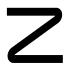
\includegraphics[keepaspectratio]{images/part001_e30b1f1b.jpg}}

多项式环 \(\mathbf{Q}[(\mathrm{X}_{n})_{n\in\mathbf{N}}]\) 是整环；它不是诺特的（也不是阿廷的）（VIII, p.~15, 习题 9）。它是它的分式域的子环，而该分式域是阿廷（且诺特）环。

\subsection{反模}

定义 3. --- 设 A 为环，M 为 A-模，\(E = \text{End}_{A}(M)\) 为 M 的自同态环。M 的反模是与 M 具有相同底层加群、外律为 \((c, x) \mapsto c(x)\) 的左 E-模。

设 Z 为环 A 的中心。对每个 \(a \in Z\) ，位似 \(a_{M}\) 属于 E。因此，E 典范地带有 Z-代数结构。特别地，若 M 是有限生成的 Z-模，则 M 的反模是有限生成的。

引理 4. --- 设 M 为反模有限生成的左 A-模。则存在自然数 m 以及一个单 \(A_{M}\) -线性映射，它从 \((\mathrm{A}_{\mathrm{M}})_{s}\) 映到 \(M^{m}\) 。

置 \(\mathrm{E}=\mathrm{End}_{\mathrm{A}}(\mathrm{M})\) 。设 \((x_{1},\ldots,x_{m})\) 为 E-模 M 的有限生成族。映射 \(\varphi:a\mapsto(ax_{1},\ldots,ax_{m})\) 把 \((\mathrm{A}_{\mathrm{M}})_{s}\) 映到 \(M^{m}\) ，它是 \(A_{M}\) -线性的。设 a 为 \(A_{M}\) 的元素且 \(\varphi(a)=0\) 。M 中使 ax = 0 的元素 x 组成的集合是 M 的包含 \(x_{1}, \ldots, x_{m}\) 的 E-子模，因此等于 M，由此推出 a = 0。

命题 6. --- 设 M 为反模有限生成的阿廷（相应地，诺特）左 A-模。则 M 的位似环 \(A_{M}\) 是左阿廷（相应地，左诺特）的。

这由引理 4 及 VIII, p.~3 的命题 3 得出。

推论. --- 设 A 为交换环。

\begin{enumerate}
\def\labelenumi{\alph{enumi})}
\item
  设 M 为诺特 A-模。则环 \(A_{M}\) 是诺特的。
\item
  设 M 为有限长度的 A-模。则环 \(A_{M}\) 是阿廷的。
\end{enumerate}

设 M 为 A-模。在 a) 或 b) 的假设下，A-模 M 是有限生成的。由于 A 交换，\(A_{M}\) 含于环 \(\operatorname{End}_{\mathrm{A}}(\mathrm{M})\) ，故 M 的反模是有限生成的。于是只需应用命题 6。

注. --- 设 A 为环。反模有限生成的阿廷左 A-模具有有限长度：事实上，M 的位似环 \(A_{M}\) 是左阿廷的（命题 6），而 M 是 \(A_{M}\) 上的阿廷模；由 VIII, p.~7 的命题 4，模 M 在 \(A_{M}\) 上具有有限长度，因而在 A 上亦然。

特别地，交换环上的每个有限生成阿廷模都具有有限长度。与此相对照，非交换环上的有限生成阿廷模不一定具有有限长度（VIII, p.~16, 习题 12）。

\subsection{诺特环上系数的多项式}

设 A 为环，\(\sigma\) 为环 A 的自同态，d 为 A 的加群的自同态，满足关系

\[
d (a b) = \sigma (a) d (b) + d (a) b\tag{1}
\]

其中 \(a, b \in A\) 任意。换句话说，d 是从环 A 到 (A,A)-双模的一个导子，该双模是在 A 的加群上赋予左作用律 \((a, x) \mapsto \sigma(a)x\) 和右作用律 \((x, a) \mapsto xa\) 而得到的。我们有 \(d(1) = 0\) （III, §10, No.~5, p.~557, 命题 3）。

回顾（IV, §1, No.~1, p.~2）A{[}X{]} 表示系数在 A 中的一元多项式组成的 Z-模 \(A \otimes_{Z} Z[X]\) 。我们赋予它左 A-模的自然结构。族 \((\mathrm{X}^{n})_{n \in \mathbf{N}}\) 是 A{[}X{]} 在 A 上的一个基。我们把 A 与它在映射 \(a \mapsto a \otimes 1\) 下的像等同起来。

命题 7. --- 设 A、\(\sigma\) 、\(d\) 如上。在群 A{[}X{]} 上存在唯一的环结构，具有下列性质：

\begin{enumerate}
\def\labelenumi{\alph{enumi})}
\item
  此环中的加法是 A{[}X{]} 的通常加法。
\item
  此环中的乘法延拓 A 的乘法。
\item
  在此环中，由 A 的一个元素 a 后接 n 个等于 X 的项组成的序列 \((a,X,\ldots,X)\) 的乘积是多项式 \(aX^{n}\) 。
\item
  在此环中，\(\mathrm{X}a = \sigma(a)\mathrm{X} + d(a)\) 对每个 \(a \in \mathrm{A}\) 成立。
\end{enumerate}

设 E 为加群 A{[}X{]} 的自同态环。把 \(a \in A\) 送到位似 \(a_{M}\) ——即左 A-模 M = A{[}X{]} 的位似——的映射，是从 A 到 E 的环同态。考虑 E 的元素 u、\(\sigma_{M}\) 与 \(d_{M}\) ，它们由 \(u(\sum b_{n}X^{n}) = \sum b_{n}X^{n+1}\) ，\(\sigma_{\mathrm{M}}(\sum b_{n}X^{n}) = \sum \sigma(b_{n})X^{n}\) ，\(d_{\mathrm{M}}(\sum b_{n}X^{n}) = \sum d(b_{n})X^{n}\) 定义。对每个 \(a \in A\) ，我们有

\[
u a _ {\mathrm{M}} = a _ {\mathrm{M}} u, \quad \sigma_ {\mathrm{M}} a _ {\mathrm{M}} = \sigma (a) _ {\mathrm{M}} \sigma_ {\mathrm{M}}, \quad d _ {\mathrm{M}} a _ {\mathrm{M}} = \sigma (a) _ {\mathrm{M}} d _ {\mathrm{M}} + (d (a) _ {\mathrm{M}}).\tag{2}
\]

\[
X_ {M} = \sigma_ {M} u+ d_ {M} .\tag{3}
\]

由 (2) 推出，对每个 \(a \in \mathbf{A}\) ，有

\[
\mathrm{X} _ {\mathrm{M}} a _ {\mathrm{M}} = \sigma (a) _ {\mathrm{M}} \mathrm{X} _ {\mathrm{M}} + (d (a) _ {\mathrm{M}}).\tag{4}
\]

考虑映射 \(\varphi : \mathrm{A}[\mathrm{X}] \to \mathrm{E}\) ，它由

\[
\varphi \Bigl (\sum a _ {n} \mathrm{X} ^ {n} \Bigr) = \sum (a _ {n}) _ {\mathrm{M}} (\mathrm{X} _ {\mathrm{M}}) ^ {n}.\tag{5}
\]

定义。这是一个群同态。一个归纳论证表明，\((\mathrm{X}_{\mathrm{M}})^{n}(1)=\mathrm{X}^{n}\) 对每个 \(n\in N\) 成立。于是 \(\varphi(\mathrm{P})(1)=\mathrm{P}\) 对每个 \(P\in\mathrm{A}[X]\) 成立，这就证明同态 \(\varphi\) 是单的。我们用 B 表示它的像。集合 B 是 E 的子群；它包含 1，并且对 \(a_{M}\) （\(a\in A\)）和 \(X_{M}\) 的左乘法封闭（见 (4)）。因此它是 E 的子环。A{[}X{]} 上由经 \(\varphi\) 的结构转移从 B 的环结构导出的唯一环结构具有命题 7 的性质，其中性质 d) 由关系 (4) 得出。

若 A{[}X{]} 带有一个具有命题 7 的性质的环结构，则此环的左位似 \(\gamma_{X}\) （I, §8, No.~1, p.~97）必然把 \(bX^{n}\) 送到 \(\sigma(b)\mathrm{X}^{n+1} + d(b)\mathrm{X}^{n}\) （对 \(b \in A\) 和 \(n \in N\) ），故等于 \(X_{M}\) 。位似 \(\gamma_{a}\) 必然等于 \(a_{M}\) ，对每个 \(a \in A\) 。于是，\(\gamma_{\mathrm{P}} = \varphi(\mathrm{P})\) 对每个 \(P \in A[X]\) 成立；命题 7 中的唯一性由此得出。

带有具有命题 7 的性质的唯一环结构的集合 A{[}X{]} 记作 \(A[X]_{\sigma,d}\) ，称为 X 的、系数在 A 中且相对于 \(\sigma\) 与 d 的多项式环。~当 d 是零映射时，我们简记为 \(A[X]_{\sigma}\) ；记号 A{[}X{]} 则用于进而 \(\sigma\) 是 A 上的恒等映射的情形。这一记号与 IV, §1, No.~1, p.~1 对交换环 A 引入的记号相容。

注. --- 环 \(A[X]_{\sigma,d}\) 具有下列泛性质：给定环 \(A'\) 、环同态 \(f: A \to A'\) 以及 \(A'\) 的元素 x，使得 \(xf(a) = f(\sigma(a))x + f(d(a))\) 对每个 \(a \in A\) 成立，则存在唯一的环同态 \(g: A[X]_{\sigma,d} \to A'\) ，它延拓 f 且把 X 映到 x。

唯一性是明显的。因此我们来证明映射 \(g: \mathrm{A}[\mathrm{X}]_{\sigma,d} \to \mathrm{A}'\) （它由 \(g(\sum a_n\mathrm{X}^n) = \sum f(a_n)x^n\) 定义）具有所需的性质。它延拓 \(f\) ，把 \(\mathrm{X}\) 映到 \(x\) ，且是群同态。我们有 \(g(1) = 1\) 。对 \(a \in \mathrm{A}\) 以及 \(\mathrm{Q} = \sum a_n\mathrm{X}^n\) （其中 Q 属于 \(\mathrm{A}[\mathrm{X}]_{\sigma,d}\) ），有

\[
g (a \mathrm{Q}) = g \left(\sum a a _ {n} X ^ {n}\right) = \sum f (a a _ {n}) x ^ {n} = f (a) \sum f (a _ {n}) x ^ {n} = g (a) g (\mathrm{Q})
\]

以及

\[
\begin{array}{l} g (\mathrm{XQ}) = g \Bigl (\sum \Bigl (\sigma (a _ {n}) \mathrm{X} ^ {n + 1} + d (a _ {n}) \mathrm{X} ^ {n} \Bigr) \Bigr) \\ = \sum (f (\sigma (a _ {n})) x ^ {n + 1} + f (d (a _ {n})) x ^ {n}) = x \sum f (a _ {n}) x ^ {n} = g (\mathrm{X}) g (\mathrm{Q}). \end{array}
\]

由此推出，\(g(\mathrm{P})g(\mathrm{Q}) = g(\mathrm{PQ})\) 对 \(A[X]_{\sigma,d}\) 中的 P、Q 成立，因而 g 是环同态。

定理 2. --- 设 A 是左诺特环，\(\sigma\) 是 A 的一个自同构，\(d\) 是 A 的加法群的一个满足关系式 (1) 的自同态。则环 \(\mathrm{A}[\mathrm{X}]_{\sigma,d}\) 是左诺特的。

令 \(B = A[X]_{\sigma,d}\) 。对任意整数 \(n \geqslant 0\) ，我们用 \(B_{n}\) 表示 B 中形如 \(a_{0} + a_{1}X + \cdots + a_{n}X^{n}\) 的元素组成的集合。它是 B 的一个左 A-子模。映射 \(\varphi_{n}: B_{n} \to A_{s}\) （由 \(\varphi_{n}(a_{0} + a_{1}X + \cdots + a_{n}X^{n}) = a_{n}\) 定义）是 A-线性的。

设 \(\mathfrak{b}\) 是 B 的一个左理想。对每个整数 \(n \geqslant 0\) ，集合 \(\mathfrak{a}_n = \varphi_n(\mathfrak{b} \cap \mathrm{B}_n)\) 是 A 的一个左理想。由于 \(Xa = \sigma(a)X + d(a)\) 对每个 \(a \in A\) 成立，我们有

\[
\varphi_ {n + 1} (\mathrm{XQ}) = \sigma (\varphi_ {n} (\mathrm{Q}))\tag{6}
\]

对每个 \(Q \in B_{n}\) 成立，因而 \(\sigma(\mathfrak{a}_{n}) \subset \mathfrak{a}_{n+1}\) 。于是，A 的理想序列 \(\mathfrak{a}_{n}^{\prime} = \sigma^{-n}(\mathfrak{a}_{n})\) 是递增的。由于环 A 是左诺特的，存在整数 \(m \geqslant 0\) ，使得 \(\mathfrak{a}_{n}^{\prime} = \mathfrak{a}_{n+1}^{\prime}\) 对 \(n \geqslant m\) 成立。由于

\(\sigma\) 是满射，我们有关系式

\[
\sigma (\mathfrak {a} _ {n}) = \mathfrak {a} _ {n + 1}\tag{7}
\]

对每个整数 \(n \geqslant m\) 成立。

设 \(\mathfrak{c}\) 是 B 的由 \(\mathfrak{b} \cap \mathrm{B}_m\) 生成的左理想。由于左 A-模 \(\mathrm{B}_m\) 是有限生成的且环 A 是左诺特的，左 A-模 \(\mathfrak{b} \cap \mathrm{B}_m\) 是有限生成的（VIII, p.~7, 命题 4 a)）。因此左理想 \(\mathfrak{c}\) 由 B 的一个有限子集生成。显然它含于 \(\mathfrak{b}\) 。我们来证明它等于 \(\mathfrak{b}\) ，办法是用归纳法证明对每个整数 \(n \geqslant 0\) 有

\[
\mathfrak {b} \cap \mathrm{B} _ {n} \subset \mathfrak {c}.\tag{8}
\]

关系式 (8) 对 \(n \leqslant m\) 按构造即成立。以下设 n 是一个整数 \(\geqslant m\) 且满足 \(b \cap B_{n} \subset c\) 。设 P 是 \(b \cap B_{n+1}\) 的一个元素。那么 \(\varphi_{n+1}(P)\) 属于 \(\mathfrak{a}_{n+1} = \sigma(\mathfrak{a}_{n})\) ，因而存在 \(b \cap B_{n}\) 的一个元素 Q，使得 \(\varphi_{n+1}(P) = \sigma(\varphi_{n}(Q))\) 。令 R = P - XQ。由关系式 (6)，我们有 \(\varphi_{n+1}(R) = 0\) ，即 \(R \in B_{n}\) 。由于 P 与 Q 都属于 B 的左理想 b，R 亦然；于是 R 与 Q 属于 \(b \cap B_{n}\) ，而由归纳假设它含于理想 c。因此 P 属于 c。~这就证明了 \(b \cap B_{n+1} \subset c\) 。

由此推出 \(\mathfrak{b}\) 等于 \(\mathfrak{c}\) ；因此它是 B 的一个有限生成理想。这就证明了环 B 是左诺特的。

如果环 A 的自同态 \(\sigma\) 不是自同构，那么环 \(A[X]_{\sigma,d}\) 不一定是左诺特的，即使 A 是诺特交换环时也是如此（VIII, p.~22, 习题 26）。

推论 1（希尔伯特）. --- 设 A 是诺特交换环。对每个整数 \(n \geqslant 0\) ，多项式代数 \(A[X_{1}, \ldots, X_{n}]\) 是诺特环。

这由定理 2 并顾及 III, §2, No.~9, p.~453 的命题 8 经归纳法得出。

推论 2. --- 设 A 是诺特交换环。由有限多个元素生成的交换 A-代数是诺特环。

这样的代数同构于形如 \(A[X_{1},\ldots,X_{n}]/\mathfrak{a}\) 的代数，其中 \(n \geqslant 0\) 且 a 是 \(A[X_{1},\ldots,X_{n}]\) 的一个理想。然后应用推论 1 以及 VIII, p.~7 的命题 5。

推论 3. --- 每个交换环都是一族右向有向的诺特子环的并。

事实上，设 A 是交换环。A 的由有限多个元素（作为 Z-代数）生成的子环由推论 2 知是诺特的。它们构成 A 的一族右向有向的子环，其并为 A。

\BourbakiExercises{习题}

\begin{enumerate}
\def\labelenumi{\arabic{enumi})}
\tightlist
\item
  设 A 是一个不是体的主理想整环，P 是由 A 的不可约元素组成的一个代表系。A-模 M 是阿廷的，当且仅当它是挠模且存在 P 的一个有限子集 S，使得下列两个条件被满足：
\end{enumerate}

\begin{enumerate}
\def\labelenumi{(\roman{enumi})}
\item
  对每个 \(\pi \in \mathrm{P} - \mathrm{S}\) ，\(\pi\) -准素分量 \(\mathrm{M}_{\pi}\) （即 \(\mathrm{M}\) 的该分量，见 VII, §2, No.~2, p.~8）均归结为 0。
\item
  对每个 \(\pi\in S\) ，被 \(\pi\) 零化的 M 中元素组成的集合，视为体 A/ \(\pi\) A 上的向量空间，是有限维的。
\end{enumerate}

\begin{enumerate}
\def\labelenumi{\arabic{enumi})}
\setcounter{enumi}{1}
\tightlist
\item
  设 A 是环，M 是长度为 n 的有限长度 A-模，R 是 M 的一族对复合封闭的幂零自同态。
\end{enumerate}

\begin{enumerate}
\def\labelenumi{\alph{enumi})}
\item
  若 n = 1，则 R 的每个元素均为零。若 n \textgreater{} 1，证明存在 M 的一个子模 N，它异于 0 与 M，且在 R 的所有元素下稳定。（可以假设 R 有一个元素 \(s \neq 0\) ；选取一个使 \(s(M)\) 具有最小长度的，并证明 srs = 0 对每个 \(r \in R\) 成立。由此推出：可取 \(N = s(M)\) （若 \(Rs = \{0\}\) ），或取 \(N = \sum_{r \in R} r(s(M))\) （若 \(Rs \neq \{0\}\) 。）\(^{(1)}\)
\item
  由 a) 推出，存在 M 的一个若尔当--赫尔德列 \((\mathrm{M}_{i})_{0\leqslant i\leqslant n}\) ，使得 \(r(\mathrm{M}_{i})\subset\mathrm{M}_{i+1}\) 对所有 \(r\in R\) 及 \(0\leqslant i\leqslant n-1\) 成立。再推出：\(r_{1}\cdots r_{n}=0\) 对 R 的 n 个元素的每个序列 \((r_{i})_{1\leqslant i\leqslant n}\) 成立。
\end{enumerate}

\begin{enumerate}
\def\labelenumi{\arabic{enumi})}
\setcounter{enumi}{2}
\tightlist
\item
  \begin{enumerate}
  \def\labelenumii{\alph{enumii})}
  \tightlist
  \item
    给出一个交换域 K 的例子，以及一个同构 \(\varphi\) ，它从 K 映到 K 的某个子域 \(K'\) ，使得 K 在 \(K'\) 上是有限维的。在加法群 \(A = K \times K\) 上，我们通过令 \((x, y)(x', y') = (xx', xy' + y\varphi(x'))\) 定义一个环结构（II, §1, p.~382, 习题 7）。A 的左理想只有 \(\{(0, 0)\}\) 、 \(\{0\} \times K\) 以及 A，但对 K 的每个 \(K'\) -线性子空间 E，\(\{0\} \times E\) 都是 A 的右理想。由此推出 A 是左阿廷且左诺特的，但既非右阿廷也非右诺特。b) 给出一个有限长度模的例子，其自同态环既非左阿廷也非左诺特。
  \end{enumerate}
\end{enumerate}

\begin{enumerate}
\def\labelenumi{\alph{enumi})}
\setcounter{enumi}{2}
\tightlist
\item
  利用与 a) 相同的方法，给出一个左、右皆阿廷的环的例子，使其左长度异于右长度。
\end{enumerate}

\begin{enumerate}
\def\labelenumi{\arabic{enumi})}
\setcounter{enumi}{3}
\tightlist
\item
  设 \(\rho : \mathrm{A} \to \mathrm{B}\) 是一个环同态。
\end{enumerate}

\begin{enumerate}
\def\labelenumi{\alph{enumi})}
\item
  如果 B 作为右 A-模是自由的且非零，且环 B 是左阿廷的（相应地，左诺特的），那么环 A 是左阿廷的（相应地，左诺特的）。
\item
  给出一个例子，其中 A 是交换域，B 作为 A 上的右向量空间是有限维的，而 B 既非左阿廷也非左诺特（利用习题 3）。
\end{enumerate}

\begin{enumerate}
\def\labelenumi{\arabic{enumi})}
\setcounter{enumi}{4}
\item
  设 n 是一个整数 \(\geqslant 1\) 。环 A 是左阿廷的（相应地，左诺特的），当且仅当矩阵环 \(\mathbf{M}_{n}(\mathrm{A})\) 是左阿廷的（相应地，左诺特的）。若 A 是左阿廷的，则 \(\mathbf{M}_{n}(\mathrm{A})\) 的左长度等于 A 的左长度的 n 倍。
\item
  设 \(A\) 是环，\(e\) 是 \(A\) 中的一个幂等元。
\end{enumerate}

\begin{enumerate}
\def\labelenumi{\alph{enumi})}
\item
  设 \(\mathfrak{a}_1\) 是环 \(e\mathrm{A}e\) 的一个左理想，\(\mathfrak{a}\) 是 A 的由 \(\mathfrak{a}_1\) 生成的左理想。我们有 \(\mathfrak{a}_1 = e\mathfrak{a}e = \mathfrak{a} \cap e\mathrm{A}e\) 。
\item
  对 A 的每个左理想 a，有 \(a \cap eAe \subset eae\) ；给出一个使这是严格包含的例子（取 A 为矩阵环）。
\item
  对 A 的每个双边理想 a，有 \(a \cap eAe = eae\) 。
\item
  若环 A 是左阿廷的（相应地，左诺特的），则环 eAe 与 \((1-e)\mathrm{A}(1-e)\) 亦然。
\item
  给出一个例子，其中 eAe 与 \((1-e)\mathrm{A}(1-e)\) 都是交换域，而 A 容许双边理想的无穷严格递增序列与无穷严格递降序列。（取一个交换域 K 上的无限维向量空间 V，给加法群 \(A=K\times V\times K\) 赋予由 \((\lambda,x,\mu)(\lambda',x',\mu')=(\lambda\lambda',\lambda x'+\mu'x,\mu\mu')\) 定义的环结构，并令 \(e=(1,0,0)\) 。）
\end{enumerate}

\begin{enumerate}
\def\labelenumi{\arabic{enumi})}
\setcounter{enumi}{6}
\tightlist
\item
  \begin{enumerate}
  \def\labelenumii{\alph{enumii})}
  \tightlist
  \item
    设 A 是一个环， \(\mathcal{I}\) 是 A 中形如 \(Ae\) 的左理想组成的集合，其中 \(e\) 是 A 中的一个幂等元。证明下列性质等价：
  \end{enumerate}
\end{enumerate}

\begin{enumerate}
\def\labelenumi{(\roman{enumi})}
\item
  \(\mathcal{I}\) 的每个非空子集都有极小元。
\item
  \(\mathcal{I}\) 的每个非空子集都有极大元。
\item
  不存在 \(\mathcal{I}\) 中非零理想组成的无限族，使其和为直和。
\item
  不存在 A 中非零幂等元组成的无限族 \((e_i)\) ，使得 \(e_i e_j = 0\) 对 \(i \neq j\) 成立。
\end{enumerate}

\begin{enumerate}
\def\labelenumi{\alph{enumi})}
\setcounter{enumi}{1}
\item
  给出一个环 A 的例子，使其中每个由单生成左理想组成的非空集都有极大元和极小元（从而 \(a\) ) 中的等价条件得到满足），尽管 A 既非左阿廷又非左诺特（利用习题 3）。
\item
  设 M 是一个模。若 M 的有限生成子模组成的每个非空集都有极大元，则 M 是诺特的。
\item
  给出一个非阿廷模的例子，使其中每个由有限生成子模组成的非空集都有极小元。
\end{enumerate}

\begin{enumerate}
\def\labelenumi{\arabic{enumi})}
\setcounter{enumi}{7}
\item
  设 A 是环，B 与 D 是 A 的两个子环。证明：若 D 是体且环 B 是左阿廷的，则 \(B \cap D\) 是体。
\item
  设 A 是非零交换环，I 是无限集。环 \(\mathrm{A}[(\mathrm{X}_{i})_{i\in\mathrm{I}}]\) 与 \(\mathrm{A}[[(\mathrm{X}_{i})_{i\in\mathrm{I}}]]\) 都既非阿廷也非诺特。
\item
  设 A 是环，a 与 b 是 A 的两个双边理想。若环 A/a 与 A/b 都是左阿廷的（相应地，左诺特的），则环 A/a∩b 亦然；与此相对，环 A/ab 不一定是左阿廷的（相应地，左诺特的）。
\item
  设 A、B 是环，M 是有限生成的左 A-模，P 是有限生成的右 A-模，N 是一个 (A, B)-双模。若右 B-模 N 是阿廷的（相应地，诺特的），则右 B-模 \(\operatorname{Hom}_{\mathrm{A}}(\mathrm{M}, \mathrm{N})\) 与 \(P \otimes_{A} N\) 亦然。
\item
  设 \(\mathrm{K}\) 是交换域。用 \((e_n)_{n\in \mathbf{N}}\) 表示向量空间 \(\mathrm{V} = \mathrm{K}^{(\mathbf{N})}\) 的典范基。我们通过令下式来定义自同态的序列 \((u_n)_{n\in \mathbf{N}}\) （它们都是 \(\mathrm{V}\) 的自同态）：
\end{enumerate}

\[
\begin{array}{l l} u _ {0} (e _ {0}) = 0 & \qquad u _ {0} (e _ {1}) = 0 \qquad u _ {0} (e _ {n + 1}) = e _ {n} \text { for } n \geqslant 1 \\ u _ {m} (e _ {0}) = e _ {m} & \qquad u _ {m} (e _ {n}) = 0 \text { for } m \geqslant 1 \text { and } n \geqslant 1. \end{array}
\]

设 \(\mathrm{A}\) 是 \(\operatorname{End}_{\mathrm{K}}(\mathrm{V})\) 的由序列 \((u_n)_{n \in \mathbf{N}}\) 生成的含幺 K-子代数。证明左 A-模 \(\mathrm{V}\) 是阿廷的、有限生成的（甚至是单生成的），但不是诺特的。

\begin{enumerate}
\def\labelenumi{\arabic{enumi})}
\setcounter{enumi}{12}
\tightlist
\item
  \begin{enumerate}
  \def\labelenumii{\alph{enumii})}
  \tightlist
  \item
    设 \(\rho: \mathrm{A} \to \mathrm{B}\) 是环同态。假设 A 是左诺特的，且存在 B 的一个有限子集 S，其元素彼此交换且与 \(\rho(\mathrm{A})\) 的元素交换，使得环 B 由 \(\rho(\mathrm{A})\) 与 S 生成。则 B 是左诺特的。
  \end{enumerate}
\end{enumerate}

\begin{enumerate}
\def\labelenumi{\alph{enumi})}
\setcounter{enumi}{1}
\tightlist
\item
  设 A 是非零交换环。给出一个结合含幺 A-代数的例子，它由有限多个元素生成，而作为环既非左诺特也非右诺特（考察自由结合代数 \(\operatorname{Libas}_{\mathrm{A}}(\mathrm{I})\) （III, §2, No.~7, p.~449, 定义 2），其中 I 是基数 \(\geqslant 2\) 的集合）。
\end{enumerate}

\begin{enumerate}
\def\labelenumi{\arabic{enumi})}
\setcounter{enumi}{13}
\tightlist
\item
  设 V 是体 K 上可数无限维的向量空间。V 的有限秩自同态组成的集合 I 是环 \(B = \text{End}_{K}(V)\) 的一个双边理想。证明环 \(A = B/I\) 的双边理想只有 \(\{0\}\) 与 A，但 A 既非左诺特也非右诺特。
\end{enumerate}

¶ 15) 设 A 是交换环，M 是有限生成的 A-模。

\begin{enumerate}
\def\labelenumi{\alph{enumi})}
\item
  假设对 A 的理想的每个递增序列 \((\mathfrak{a}_{n})_{n\in\mathbf{N}}\) ，序列 \((\mathfrak{a}_{n}\mathrm{M})_{n\in\mathbf{N}}\) 都是平稳的。证明 A-模 M 是诺特的。（化归到 A-模 M 忠实、且对 A 的每个理想 \(a\neq0\) ，A-模 M/aM 都是诺特的情形。此时存在 M 的一个子模 \(N_{0}\) ，它在使 M/N 忠实的子模 \(N\subset M\) 当中是极大的。证明 A-模 \(M/N_{0}\) 是诺特的，再证明环 A 是诺特的，并由此完成证明。）
\item
  *假设对 A 的理想的每个递降序列 \((\mathfrak{a}_n)_{n \in \mathbf{N}}\) ，序列 \((\mathfrak{a}_n\mathrm{M})_{n \in \mathbf{N}}\) 都是平稳的。证明 A-模 M 是阿廷的。（化归到 A-模 M 忠实的情形。证明此时 A 只有有限多个极大理想，并且借助 VIII, p.~173 命题 1 的证明可知 A 的根是幂零的。推出存在 A 的极大理想的一个有限序列 \((\mathfrak{m}_{1}, \mathfrak{m}_{2}, \cdots, \mathfrak{m}_{n})\) ，其乘积零化 M。对 \(n.)_{*}\) 作归纳来完成证明。）
\end{enumerate}

\begin{enumerate}
\def\labelenumi{\arabic{enumi})}
\setcounter{enumi}{15}
\tightlist
\item
  \begin{enumerate}
  \def\labelenumii{\alph{enumii})}
  \tightlist
  \item
    设 A 是交换环，\(\rho: A \to B\) 是单射环同态，它使 B 成为有限生成的左 A-模。假设对 A 的理想的每个递增（相应地，递降）序列 \((\mathfrak{a}_{n})_{n \in \mathbf{N}}\) ，序列 \((\mathfrak{a}_{n}B)_{n \in \mathbf{N}}\) 都是平稳的（若环 B 是右诺特的（相应地，右阿廷的），则即属此情形）。证明环 A 是诺特的（相应地，阿廷的）（利用习题 15）。
  \end{enumerate}
\end{enumerate}

\begin{enumerate}
\def\labelenumi{\alph{enumi})}
\setcounter{enumi}{1}
\tightlist
\item
  给出一个左、右皆阿廷且诺特的环 B 及 B 的一个子环 A 的例子，使得 B 作为左、右 A-模都是有限生成的，而环 A 既非左也非右诺特或阿廷（选取一个适当的整环 C，其分式域为 K，取 B 为矩阵环 \(\mathbf{M}_{3}(\mathrm{K})\) ，并取 A 为 B 的由矩阵 \((a_{ij})_{1\leqslant i,j\leqslant3}\) 组成的子环，这些矩阵满足 \(a_{ij}=0\) （对 \(1\leqslant i<j\leqslant3\) ）且 \(a_{22}\in C.\) ）
\end{enumerate}

\begin{enumerate}
\def\labelenumi{\arabic{enumi})}
\setcounter{enumi}{16}
\tightlist
\item
  设 E 是一个幺半群，e 是其单位元，S 是 E 的一个子集，\(S'\) 是 E 的由 S 生成的子幺半群。我们说 S 在 E 上容许左分式演算，如果下列两个（当 E 交换时是重言式的）条件被满足：
\end{enumerate}

\begin{enumerate}
\def\labelenumi{(\roman{enumi})}
\item
  对每个 \(a \in \mathrm{E}\) 与每个 \(s \in \mathrm{S}\) ，存在 \(b \in \mathrm{E}\) 与 \(t \in \mathrm{S}'\) ，使得 \(ta = bs\) 。
\item
  对每组的 \(a \in \mathrm{E}\) 、 \(b \in \mathrm{E}\) 与 \(s \in \mathrm{S}\) ，若 \(as = bs\) ，则存在 \(t \in \mathrm{S}'\) ，使得 \(ta = tb\) 。
\end{enumerate}

\(a)\) 假设存在一个同态 \(u\) ，它从 E 映到幺半群 \(\mathrm{E}'\) ，使得 \(u(\mathrm{S})\) 的每个元素在 \(\mathrm{E}'\) 中可逆，且对 E 中的每对 \(a, b\) ，若 \(u(a) = u(b)\) ，则存在 \(s \in \mathrm{S}'\) ，使得 \(sa = sb\) 。则 S 在 E 上容许左分式演算。

\begin{enumerate}
\def\labelenumi{\alph{enumi})}
\setcounter{enumi}{1}
\item
  假设 S 在 E 上容许左分式演算。在 \(E \times S'\) 中，我们用 \((a, s) \sim (b, t)\) 表示关系``存在 E 中的 c 与 d，使得 ca = db 且 \(cs = dt \in S'\) 。''这是一个等价关系。我们令 \(S^{-1}E = (E \times S') / \sim\) ，并用 \(\varepsilon : E \to S^{-1}E\) 表示把 \(a \in E\) 映到 \((a, e)\) 的类的映射。在 \(S^{-1}E\) 上存在唯一的幺半群结构，使得 \(\varepsilon\) 是保单位元的同态，使得 \(\varepsilon(s)\) 对每个 \(s \in S\) 可逆，且使得对 \((a, s) \in E \times S'\) ，\((a, s)\) 在 \(S^{-1}E\) 中的类等于 \(\varepsilon(s)^{-1}\varepsilon(a)\) 。我们说 \(S^{-1}E\) 是 E 的相伴于 S 的左分式幺半群。当幺半群 E 交换时，它与 I, §2, No.~4, p.~18 中定义的那个一致。
\item
  设 \(a, b\) 在 E 中。\(\varepsilon(a) = \varepsilon(b)\) 成立，当且仅当存在 \(s \in S'\) ，使得 \(sa = sb\) 。映射 \(\varepsilon\) 是单射的（相应地，双射的），当且仅当 S 的每个元素是右正则的（相应地，可逆的）。
\item
  设 f 是从 E 到幺半群 F 的一个保单位元同态，使得 \(f(\mathrm{S})\) 的每个元素在 F 中可逆。存在唯一的同态 \(\overline{f}: S^{-1}E \to F\) ，使得 \(f = \overline{f} \circ s\) 。若 f 是单射，则 \(\overline{f}\) 是单射。
\item
  我们说 S 在 E 上容许右分式演算，如果它在 E 的反幺半群 \(E^{o}\) 上容许左分式演算。在这种情形，定义 E 的相伴于 S 的右分式幺半群 \(ES^{-1}\) ，注意到 \((\mathrm{ES}^{-1})^{\circ} = \mathrm{S}^{-1}(\mathrm{E}^{\circ})\) ，并对右分式幺半群改写 b)。若 S 在 E 上容许左、右分式演算，则幺半群 \(S^{-1}E\) 与 \(ES^{-1}\) 典范同构。
\end{enumerate}

\begin{enumerate}
\def\labelenumi{\arabic{enumi})}
\setcounter{enumi}{17}
\tightlist
\item
  \begin{enumerate}
  \def\labelenumii{\alph{enumii})}
  \tightlist
  \item
    设 A 是环，S 是 A 的一个子集，S' 是 A 的包含 1 与 S 且对乘法封闭的最小子集。我们说 S 在 A 上容许左分式演算，如果下列两个（当 A 交换时是重言式的）条件被满足：
  \end{enumerate}
\end{enumerate}

\begin{enumerate}
\def\labelenumi{(\roman{enumi})}
\item
  对每个 \(a \in \mathrm{A}\) 与每个 \(s \in \mathrm{S}\) ，存在 \(b \in \mathrm{A}\) 与 \(t \in \mathrm{S}'\) ，使得 \(ta = bs\) 。
\item
  对每组的 \(a \in \mathrm{A}\) 与 \(s \in \mathrm{S}\) ，若 \(as = 0\) ，则存在 \(t \in \mathrm{S}'\) ，使得 \(ta = 0\) 。
\end{enumerate}

这等价于说 S 在给集合 A 只赋予乘法而得的幺半群上容许左分式演算（习题 17）。证明：此时在乘法幺半群 \(S^{-1}A\) 上存在唯一的加法，使得赋有该加法及其乘法的 \(S^{-1}A\) 是一个环，且典范映射 \(\varepsilon: A \to S^{-1}A\) （同前所引）是环同态。我们说 \(S^{-1}A\) 是 A 的相伴于 S 的左分式环。当 A 交换时，它与 I, §8, No.~12, p.~113 中定义的环一致。

\begin{enumerate}
\def\labelenumi{\alph{enumi})}
\setcounter{enumi}{1}
\item
  集合 S 在 A 上容许左分式演算，当且仅当存在一个环 B 与一个环同态 \(u: A \to B\) ，使得 \(u(S)\) 的每个元素在 B 中可逆，且对每个 \(a \in u^{-1}(0)\) ，存在 \(s \in S\) ，使得 sa = 0。
\item
  假设 S 在 A 上容许左分式演算。典范同态 \(\varepsilon : \mathrm{A} \to \mathrm{S}^{-1}\mathrm{A}\) 的核是这样的 \(a \in \mathrm{A}\) 组成的集合：存在 \(s \in \mathrm{S}\) ，使得 \(sa = 0\) 。
\end{enumerate}

设 \(f\) 是从 A 到环 B 的一个同态，使得 \(f(\mathrm{S})\) 的每个元素在 B 中可逆。存在唯一的同态 \(\overline{f} : \mathrm{S}^{-1}\mathrm{A} \to \mathrm{F}\) ，使得 \(f = \overline{f} \circ s\) 。若 \(f\) 是单射，则 \(\overline{f}\) 是单射。

\begin{enumerate}
\def\labelenumi{\alph{enumi})}
\setcounter{enumi}{3}
\item
  对右分式演算叙述与 a)、b)、c) 类似的命题；若 S 在 A 上容许右分式演算，我们把 A 的右分式环记作 AS \(^{-1}\) 。在此情形，我们有 \((\mathrm{AS}^{-1})^{\circ} = \mathrm{S}^{-1}(\mathrm{A}^{\circ})\) 。若 S 在 A 上容许左、右分式演算，则环 S \(^{-1}\) A 与 AS \(^{-1}\) 典范同构。
\item
  设 A 是一个无零因子的非零环。则 A 容许一个左分式域（I, §9, p.~177, 习题 15），当且仅当 A 的非零元素组成的集合 S 在 A 上容许左分式演算，且在此情形，\(S^{-1}A\) 是 A 的左分式域。
\end{enumerate}

\begin{enumerate}
\def\labelenumi{\arabic{enumi})}
\setcounter{enumi}{18}
\tightlist
\item
  设 A 是环，S 是 A 的一个在 A 上容许左分式演算的子集（习题 18），S' 是 A 的包含 1 与 S 且对乘法封闭的最小子集。我们用 \(S^{-1}A\) 表示 A 的相伴于 S 的左分式环，并用 \(\varepsilon:A\to S^{-1}A\) 表示典范同态。
\end{enumerate}

\begin{enumerate}
\def\labelenumi{\alph{enumi})}
\item
  设 M 是一个 A-模。我们把 \(S^{-1}A\) -模 \(S^{-1}A \otimes_{A} M\) 记作 \(S^{-1}M\) ，并称之为 M 的相伴于 S 的左分式模。证明 \(S^{-1}M\) 的每个元素都可以写成 \(\varepsilon(s)^{-1} \otimes x\) ，其中 \(x \in M\) 且 \(s \in S'\) ；并且对 M 中的 x, y 与 \(S'\) 中的 s, t，关系 \(\varepsilon(s)^{-1} \otimes x = \varepsilon(t)^{-1} \otimes y\) 等价于存在 A 的一对元素 \((c, d)\) ，使得 cx = dy 且 \(cs = dt \in S'\) 。
\item
  我们用 \(\varepsilon_{M}\) 表示典范 A-线性映射 \(x \mapsto 1 \otimes x\) （从 M 到 \(S^{-1}M\) ）。它的像生成 \(S^{-1}A\) -模 \(S^{-1}M\) ；它的核由这样的 \(x \in M\) 组成：存在 \(s \in S'\) ，使得 sx = 0。映射 \(\varepsilon_{M}\) 是单射的（相应地，双射的），当且仅当对每个 \(s \in S\) ，M 的位似 \(x \mapsto sx\) 是单射的（相应地，双射的）。
\end{enumerate}

\(c)\) \(\mathrm{S}^{-1}\mathrm{M} = 0\) 成立，当且仅当对每个 \(x\in \mathrm{M}\) ，存在 \(s\in \mathrm{S}\) ，使得 \(sx = 0\) 。

\begin{enumerate}
\def\labelenumi{\alph{enumi})}
\setcounter{enumi}{3}
\item
  设 N 是 M 的一个子模。典范 \(S^{-1}A\) -线性映射（从 \(S^{-1}N\) 到 \(S^{-1}M\) ）是单射。（*换言之，右 A-模 \(S^{-1}A\) 是平坦的。*）我们把 \(S^{-1}N\) 与它在 \(S^{-1}M\) 中此映射下的像等同。M 的子模 \(\bar{\varepsilon}_{\mathrm{M}}^{-1}(\mathrm{S}^{-1}\mathrm{N})\) 由这样的 \(x \in M\) 组成：存在 \(s \in S'\) ，使得 \(sx \in N\) 。我们说它是 N 对 S 的左饱和。
\item
  映射 \(N^{\prime} \mapsto \varepsilon_{M}^{-1}(N^{\prime})\) 是一个从 \(S^{-1}A\) -子模组成的有序集（这些子模取自 \(S^{-1}M\) ）到 M 的对 S 左饱和（即等于其饱和）的 A-子模组成的有序集上的同构。逆同构是 \(N \mapsto S^{-1}N\) 。f) 若 A-模 M 是诺特的，则 \(S^{-1}A\) -模 \(S^{-1}M\) 是诺特的。若 A-模 M 是阿廷的，则 \(S^{-1}A\) -模 \(S^{-1}M\) 是阿廷的，且映射 \(\varepsilon_{M}: M \to S^{-1}M\) 是满射。
\end{enumerate}

\(g\) ) 若环 A 是左诺特的（相应地，左阿廷的），则环 \(\mathrm{S}^{-1}\mathrm{A}\) 亦然。\(h\) ) 对右模的右分式模，叙述与本习题类似的命题。

\begin{enumerate}
\def\labelenumi{\arabic{enumi})}
\setcounter{enumi}{19}
\item
  证明一个无零因子的左诺特环 A 容许左分式域（习题 18）（若 a 与 s 是 A 的非零元素，利用理想序列 \((As + Asa + \cdots + Asa^{n})_{n \in \mathbf{N}}\) 是平稳的这一事实，证明 \(Aa \cap As\) 不归结为 0）。
\item
  设 A 是环，\(\sigma\) 是环 A 的一个自同态，\(d\) 是 A 的加法群的一个满足关系式 \(d(ab) = \sigma(a)d(b) + d(a)b\) 的幂零自同态。\(a)\) 证明集合 \(S = \{X\}\) 在环 \(B = A[X]_{\sigma,d}\) （VIII, p.~11）上容许左分式演算（习题 18）。若 \(\sigma\) 是单射，则从 B 到 \(S^{-1}B\) 的典范同态是单射，且我们把 B 与 \(S^{-1}B\) 的一个子环等同。若 \(\sigma\) 是双射，则 S 在 B 上还容许右分式演算，且 \(S^{-1}B\) 的每个元素都可以唯一地写成 \(\sum_{n\in\mathbf{Z}}a_nX^n\) ，其中 \((a_n)_{n\in\mathbf{Z}}\) 是 A 的一个有限支集的元素族。对 \(a \in \mathrm{A}\) ，把元素 \(\mathrm{X}^{-1}a\) ——它属于 \(\mathrm{S}^{-1}\mathrm{B}\) ——写成这种形式。
\end{enumerate}

\begin{enumerate}
\def\labelenumi{\alph{enumi})}
\setcounter{enumi}{1}
\item
  证明环 \(A[X]_{\sigma,d}\) 中的乘法由连续性扩张为集合 \(A[[X]]\) （系数在 A 中、关于 X 的形式幂级数的集合）上的一个乘法。赋有该乘法的加法群 \(A[[X]]\) 是一个环，我们把它记作 \(A[[X]]_{\sigma,d}\) （若 d=0，也简记为 \(A[[X]]_{\sigma}\) ）。给出一个例子，其中一个常数项等于 1 的形式幂级数 \(u\in A[[X]]\) 在环 \(A[[X]]_{\sigma,d}\) 中既无左逆也无右逆。
\item
  证明 \(A[[X]]_{\sigma}\) 的可逆元素恰是那些常数项在 A 中可逆的元素。
\item
  把环 \(A[X]_{\sigma,d}\) 换为环 \(A[[X]]_{\sigma,d}\) 之后，叙述并证明 a) 的类似命题。
\item
  设 A 是体，\(\sigma\) 是 A 的一个自同构。则 \(\mathrm{S}^{-1}\mathrm{A}[[\mathrm{X}]]_{\sigma}\) （其中 \(\mathrm{S} = \{\mathrm{X}\}\) ）是一个体，其每个元素都可以唯一地写成 \(\sum_{n\in \mathbf{Z}}a_n\mathrm{X}^n\) ，其中 \((a_{n})_{n\in \mathbf{Z}}\) 是 A 的一个元素族，其指标 \(< 0\) 的非零项只有有限多个。我们把该体记作 \(\mathrm{A}((\mathrm{X}))_{\sigma}\) 。
\end{enumerate}

\(f\) ) 设 A 是交换域。描述体 \(\mathrm{A}((\mathrm{X}))_{\sigma}\) 的中心。由此推出一个在其中心上为无限次数的体的例子。

\begin{enumerate}
\def\labelenumi{\arabic{enumi})}
\setcounter{enumi}{21}
\tightlist
\item
  设 G 是群，H 是 G 的一个正规子群，使得商群 G/H 同构于 Z。设 g 是 G 的一个元素，它在 G/H 中的典范像生成 G/H。设 C 是交换环，A 是 H 在 C 上的代数 C{[}H{]}（III, §2, No.~6, p.~446），\((e_{h})_{h\in\mathrm{H}}\) 是其典范基，\(\sigma\) 是 A 的把 \(e_{h}\) 映到 \(e_{ghg^{-1}}\) 的自同构。
\end{enumerate}

\begin{enumerate}
\def\labelenumi{\alph{enumi})}
\item
  证明存在唯一的同态 \(u\) ，它从环 \(\mathrm{B} = \mathrm{A}[\mathrm{X}]_{\sigma}\) 到环 \(\mathrm{C}[\mathrm{G}]\) ，延拓 \(\mathrm{A} = \mathrm{C}[\mathrm{H}]\) 到 \(\mathrm{C}[\mathrm{G}]\) 中的典范单射，且把 \(\mathrm{X}\) 映为元素 \(e_g\) ——后者属于 \(\mathrm{C}[\mathrm{G}]\) 的典范基。
\item
  令 \(S = \{X\}\) 。证明 u 扩张为从环 \(S^{-1}B\) （参看习题 21）到 C{[}G{]}的一个同构。由此推出：若环 C{[}H{]}是左诺特的，则环 C{[}G{]}亦然。
\end{enumerate}

\begin{enumerate}
\def\labelenumi{\arabic{enumi})}
\setcounter{enumi}{22}
\tightlist
\item
  设 A 是环，I 是集合，\(\symbf{\sigma} = (\sigma_{i})_{i \in \mathrm{I}}\) 是环 A 的一族自同态，\(\symbf{d} = (d_{i})_{i \in \mathrm{I}}\) 是 A 的加法群的一族自同态，它们满足关系式
\end{enumerate}

\[
\sigma_ {i} \circ \sigma_ {j} = \sigma_ {j} \circ \sigma_ {i} \quad \sigma_ {i} \circ d _ {j} = d _ {j} \circ \sigma_ {i} \quad d _ {i} \circ d _ {j} = d _ {j} \circ d _ {i}
\]

对 \(i\in \mathrm{I},j\in \mathrm{I},i\neq j\) 以及

\[
d _ {i} (a b) = \sigma_ {i} (a) d _ {i} (b) + d _ {i} (a) b
\]

对 \(i \in I\) ， \(a \in A\) ， \(b \in A\) 。

\begin{enumerate}
\def\labelenumi{\alph{enumi})}
\tightlist
\item
  证明存在唯一的环 B，其加法群是多项式的加法群 A{[}X{]}——这些多项式以变元族 \(\mathbf{X} = (\mathrm{X}_{i})_{i \in \mathrm{I}}\) 、系数在 A 中——且其乘法具有下列性质：
\end{enumerate}

\begin{enumerate}
\def\labelenumi{(\roman{enumi})}
\item
  B 的元素 \(\mathrm{X}_i\) （ \(i \in \mathrm{I}\) ）两两可交换。
\item
  对每个 \(a \in A\) 与每个多重指标 \(\boldsymbol{\nu} = (\nu_i)_{i \in I} \in \mathbf{N}^{(I)}\) ，a 与一个由 \(\nu_i\) 个等于 \(X_i\) （对每个 \(i \in I\) ）的元素组成的有限序列按此顺序在 B 中的乘积是多项式 \(aX^\nu\) 。
\item
  对每个 \(a \in \mathrm{A}\) 与每个 \(i \in \mathrm{I}\) ，在环 B 中有关系式 \(\mathrm{X}_i a = \sigma_i(a)\mathrm{X}_i + d_i(a)\) 。
\end{enumerate}

\begin{enumerate}
\def\labelenumi{\alph{enumi})}
\setcounter{enumi}{1}
\item
  环 B 记作 \(A[X]_{\sigma,d}\) 。它具有下列泛性质：给定环 C、环同态 \(f: A \to C\) 以及 C 的一族两两可交换的元素 \((x_i)_{i \in I}\) ，使得 \(x_i f(a) = f(\sigma_i(a)) x_i + f(d_i(a))\) 对每个 \(a \in A\) 与每个 \(i \in I\) 成立，则存在唯一的环同态 \(g: B \to C\) ，它延拓 f，且使得 \(g(X_i) = x_i\) 对 \(i \in I\) 成立。
\item
  设 J 是 I 的一个子集。把环 \(\mathrm{A}[(\mathrm{X}_{i})_{i\in\mathrm{J}}]_{(\sigma_{i})_{i\in\mathrm{J}},(d_{i})_{i\in\mathrm{J}}}\) 记作 \(B'\) 。对每个 \(i\in I-J\) ，存在唯一的自同态 \(\sigma_{i}'\) （环 \(B'\) 的）与唯一的自同态 \(d_{i}'\) （\(B'\) 的加法群的），使得
\end{enumerate}

\[
\begin{array}{l l} \sigma_ {i} ^ {\prime} (a) = \sigma_ {i} (a) & d _ {i} ^ {\prime} (a) = d _ {i} (a) \qquad \text {for a\ensuremath{\in} A}, \\ \sigma_ {i} ^ {\prime} (\mathrm{X} _ {j}) = \mathrm{X} _ {j} & d _ {i} ^ {\prime} (\mathrm{X} _ {j}) = 0 \qquad \text {for j\ensuremath{\in} J}, \\ d _ {i} ^ {\prime} (\mathrm{PQ}) = \sigma_ {i} ^ {\prime} (\mathrm{P}) d _ {i} ^ {\prime} (\mathrm{Q}) + d _ {i} ^ {\prime} (\mathrm{P}) \mathrm{Q} & \text {for P\ensuremath{\in} B , Q\ensuremath{\in} B}. \end{array}
\]

令 \(\sigma' = (\sigma_i')_{i \in \mathbf{I} - \mathbf{J}}\) ，\(d' = (d_i')_{i \in \mathbf{I} - \mathbf{J}}\) 。从 \(\mathrm{A}[(\mathrm{X}_i)_{i \in \mathbf{I}}]\) 到 \(\mathrm{A}[(\mathrm{X}_j)_{j \in \mathbf{J}}][(\mathrm{X}_i)_{i \in \mathbf{I} - \mathbf{J}}]\) 的典范双射是从环 \(\mathrm{B} = \mathrm{A}[(\mathrm{X}_i)_{i \in \mathbf{I}}]_{\sigma, d}\) 到环 \(\mathrm{B}'[(\mathrm{X}_i)_{i \in \mathbf{I} - \mathbf{J}}]_{\sigma', d'}\) 的一个同构。

\(d)\) 若环 A 是左诺特的，则集合 I 有限；且若对每个 \(i \in \mathrm{I}\) ，A 的自同态 \(\sigma_i\) 都是双射，则环 \(\mathrm{B} = \mathrm{A}[\mathbf{X}]_{\sigma,d}\) 是左诺特的。\(e)\) 假设对每个 \(i \in \mathrm{I}\) ，态射 \(\sigma_i\) 是 A 上的恒等映射。设 E 是 A 的加法群的自同态环。证明存在唯一的环同态 \(\psi\) ，它从 \(\mathrm{B} = \mathrm{A}[\mathbf{X}]_{\sigma,d}\) 到 E，使得 \(\psi(\mathrm{X}_i) = d_i\) 对 \(i \in \mathrm{I}\) 成立，且对所有 \(a \in \mathrm{A}\) ，态射 \(\psi(a)\) 是 A 的左位似 \(b \mapsto ab\) 。\(f)\) 保留 \(e)\) 的假设。再设 A 是系数在一个（不必交换的）环 C 中的多项式环 \(\mathrm{C}[(\mathrm{T}_i)_{i \in \mathrm{I}}]\) ，且对每个 \(i \in \mathrm{I}\) ，态射 \(d_i\) 是 A 的导子 \(\mathrm{P} \mapsto \frac{\partial\mathrm{P}}{\partial\mathrm{T}_i}\) 。证明：若 C 非零且在 \(\mathbf{Z}\) 上无挠，则同态 \(\psi: \mathrm{B} \to \mathrm{E}\) 是单射。证明：若 C 是特征 \(p > 0\) 的环（V, §1, No.~2, p.~2），则 \(\psi\) 的核是 B 的由元素 \(\mathrm{X}_i^p\) （ \(i \in \mathrm{I}\) ）生成的左理想。

¶ 24) 设 G 是群，e 是其单位元，A 是非零交换环。用 A{[}G{]}表示群 G 在 A 上的代数（III, §2, No.~6, p.~446）。

\begin{enumerate}
\def\labelenumi{\alph{enumi})}
\item
  设 I 是有限集，\((\mathrm{G}_{i})_{i\in\mathrm{I}}\) 是 G 的一族子群，\((g_{i})_{i\in\mathrm{I}}\) 是 G 的一族元素。证明：若 G 是族 \((g_{i}\mathrm{G}_{i})_{i\in\mathrm{I}}\) 的并，则诸子群 \(G_{i}\) 之一在 G 中有有限指数。
\item
  假设 G 中异于 \(\{e\}\) 的每个共轭类都是无限的，且环 A 是整环。证明：若 a 与 b 是环 A{[}G{]}的两个非零双边理想，则我们有 \(ab \neq 0\) 。（在 a 与 b 中选取元素 \(a = \sum a_g g\) 与 \(b = \sum b_g g\) ，满足 \(a_e \neq 0\) 与 \(b_e \neq 0\) 。利用 a) 证明：必要时把 a 换成 \(hah^{-1}\) （取适当的 \(h \in G\) ），可以假设 \(a_g b_{g^{-1}} = 0\) 对 G 中每个 \(g \neq e\) 成立。）*c) 证明环 A{[}G{]}是左（相应地，右）阿廷的，当且仅当环 A 是阿廷的且群 G 是有限的。（若 A{[}G{]}是左阿廷的，由 VIII, p.~6 的定理 1 推出群 G 有有限长度；为证明它有限，化归到 A 是体且 G 是单群的情形，然后用 b) 与 VIII, p.~173 的命题 1。）*
\end{enumerate}

\begin{enumerate}
\def\labelenumi{\arabic{enumi})}
\setcounter{enumi}{24}
\tightlist
\item
  沿用习题 24 的记号。
\end{enumerate}

\begin{enumerate}
\def\labelenumi{\alph{enumi})}
\item
  对 G 的任一子群 H，令 \(I_{H}\) 为典范满射 \(\mathbf{Z}[G] \to \mathbf{Z}^{(G/H)}\) 的核。则映射 \(H \mapsto I_{H}\) 是从 G 的子群组成的集合到 \(Z[G]\) 的左理想组成的集合的递增单射；若 H 是 G 的正规子群，则理想 \(I_{H}\) 是双边的。
\item
  假设环 A{[}G{]}是左诺特的。则它也是右诺特的。对 G 的每个子群 H，环 A{[}H{]}是左诺特的；特别地，环 A 是诺特的。若 H 在 G 中正规，则环 A{[}G/H{]}是左诺特的。G 的每个子群都容许一个有限生成系。
\item
  证明下列性质等价：
\end{enumerate}

\begin{enumerate}
\def\labelenumi{(\roman{enumi})}
\item
  群 G 容许一个合成列，其商是有限的或同构于 Z。
\item
  群 G 容许一个合成列 \((\mathrm{G}_i)_{0\leqslant i\leqslant n}\) ，使得 \(\mathrm{G}_1\) 在 G 中有有限指数，且 \(\mathrm{G}_i / \mathrm{G}_{i + 1}\) 同构于 \(\mathbf{Z}\) （对 \(0\leqslant i\leqslant n - 1\) ）。
\end{enumerate}

当这些性质成立且环 A 是诺特的时，环 A{[}G{]}是左诺特的（利用习题 22）。

\begin{enumerate}
\def\labelenumi{\arabic{enumi})}
\setcounter{enumi}{25}
\item
  设 K 是交换域，A 是多项式环 K{[}T{]}，\(\sigma\) 是环 A 的自同态 \(\mathrm{P(T)}\mapsto\mathrm{P(T^{2})}\) 。环 \(A[X]_{\sigma}\) 不是左诺特的，尽管环 A 是诺特的。
\item
  设 D 是体，\(\sigma\) 是 D 的一个自同构，\(d\) 是 D 的加法群的一个满足 VIII, p.~9 中关系式 (1) 的自同态，A 是环 \(\mathrm{D}[\mathrm{X}]_{\sigma,d}\) （VIII, p.~11）。给定 A 的一个非零元素 \(\mathrm{P} = \sum_{n}a_{n}\mathrm{X}^{n}\) ，最大的整数 \(n\) （使 \(a_{n}\neq 0\) ）称为 P 的次数，记作 \(\deg (\mathrm{P})\) 。我们令 \(\deg (0) = -\infty\) 。
\end{enumerate}

\begin{enumerate}
\def\labelenumi{\alph{enumi})}
\item
  设 F, G 是 A 的元素且 \(G \neq 0\) ；证明存在 A 的完全确定的元素 Q, R（相应地， \(Q', R'\) ），使得 \(F = QG + R\) 且 \(\deg(R) < \deg(G)\) （相应地， \(F = GQ' + R'\) 且 \(\deg(R') < \deg(G)\) ）。
\item
  由此推出 A 的每个左（相应地，右）理想都是单生成的。若 F, G, H, K 是 A 的满足 AF + AG = AH 与 AF ∩ AG = AK 的元素，则我们有 \(\deg(\mathrm{F}) + \deg(\mathrm{G}) = \deg(\mathrm{H}) + \deg(\mathrm{K})\) （注意到 D-向量空间 A/AF 的维数是 \(\deg(\mathrm{F})\) ）。
\item
  A 的理想 AF 是极大的，当且仅当 F 不可约，即 F 不是两个非常数多项式的乘积。
\end{enumerate}

\begin{enumerate}
\def\labelenumi{\arabic{enumi})}
\setcounter{enumi}{27}
\tightlist
\item
  设 B 是环，A 是 B 的一个子环，x 是 B 的一个元素，使得 \(A + Ax = A + xA\) ，且环 B 由 \(A \cup \{x\}\) 生成。
\end{enumerate}

\begin{enumerate}
\def\labelenumi{\alph{enumi})}
\item
  设 M 是诺特的左 A-模；证明 B-模 \(\mathrm{M}_{(\mathrm{B})} = \mathrm{B} \otimes_{\mathrm{A}} \mathrm{M}\) 是诺特的。特别地，若环 A 是左诺特的，则 B 亦然。
\item
  设 A-模 M 有有限长度 n；证明 \(\mathrm{M}_{(\mathrm{B})}\) 的每个 B-子模都容许一个基数 \(\leqslant n\) 的生成子集（改编 VIII, p.~6 的定理 1 的证明）。
\end{enumerate}

\section{有限长度模的结构}

\subsection{局部环}

命题 1. --- 设 A 是非零环，r 是 A 的不可逆元素组成的集合。下列性质等价：

\begin{enumerate}
\def\labelenumi{(\roman{enumi})}
\item
  集合 \(\mathfrak{r}\) 是 A 的一个双边理想。
\item
  集合 \(\mathfrak{r}\) 对加法封闭。
\item
  环 A 有唯一的极大左理想。
\item
  对每个 \(a \in \mathbf{A}\) ，元素 \(a\) 与 \(1 - a\) 之一可逆。
\item
  对每个 \(a \in \mathbf{A}\) ，元素 \(a\) 与 \(1 - a\) 之一左可逆。
\end{enumerate}

蕴涵关系 (i) \(\Rightarrow\) (ii) 由理想的定义得出。由于 1 不属于 \(\mathfrak{r}\) ，我们有 (ii) \(\Rightarrow\) (iv)。

我们有 \(\mathfrak{r} \neq \mathrm{A}\) ，且集合 \(\mathfrak{r}\) 包含 \(\mathrm{A}\) 的每个不等于 \(\mathrm{A}\) 的左理想。若 \(\mathfrak{r}\) 是 \(\mathrm{A}\) 的一个左理想，则它因此是 \(\mathrm{A}\) 的唯一极大左理想。这就证明了 (i) 蕴涵 (iii)。

设 A 有唯一的极大左理想 m。取 \(b \in A - m\) 。左理想 Ab 不含于 A 的任何极大左理想，因此等于 A（I, §8, No.~6, p.~104, 定理 1），于是 b 左可逆。对每个 \(a \in A\) ，元素 a 与 1 - a 之一属于 A - m，因为 m 是一个不含 1 的理想。于是 (iii) 蕴涵 (v)。

设性质 (v) 成立。设 b 是 A 的一个左可逆元素。取 \(c \in A\) 使得 cb = 1。我们有 \((1 - bc)b = 0\) 且 \(b \neq 0\) ；因此 1 - bc 不是左可逆的。由性质 (v)，bc 左可逆，从而 c 更是左可逆的。于是 c 可逆；b 是它的逆，故 b 可逆。由此得出 (v) 蕴涵 (iv)。

剩下要证明 (iv) 蕴涵 (i)。设 (iv) 成立。则由下列断言 a) 至 d)，\(\mathfrak{r}\) 是 A 的一个双边理想：

\begin{enumerate}
\def\labelenumi{\alph{enumi})}
\item
  我们有 \(0 \in \mathfrak{r}\) ，因为环 A 非零。
\item
  A 的两个元素——一个属于 r，另一个属于 A-r——的乘积属于 r。
\item
  集合 \(\mathfrak{r}\) 对加法封闭。
\end{enumerate}

事实上，设 \(a\) 与 \(b\) 是 \(\mathfrak{r}\) 的元素，使得 \(s = a + b\) 可逆。由 b)，A 的元素 \(s^{-1}a\) 与 \(s^{-1}b\) 都属于 \(\mathfrak{r}\) ；由于 \(s^{-1}b = 1 - s^{-1}a\) ，这与 (iv) 成立的假设矛盾。

\begin{enumerate}
\def\labelenumi{\alph{enumi})}
\setcounter{enumi}{3}
\tightlist
\item
  集合 \(\mathfrak{r}\) 对乘法封闭。
\end{enumerate}

事实上，设 \(a\) 与 \(b\) 是 \(\mathfrak{r}\) 的两个元素。元素 \(a' = -a(1 - b)\) 属于 \(\mathfrak{r}\) （由 \(\mathrm{b}\) )），于是元素 \(ab\) ——它等于 \(a + a'\) ——属于 \(\mathfrak{r}\) （由 \(\mathrm{c}\)）；断言 d) 得证。

定义 1. --- 局部环是一个具有命题 1 中诸等价性质的非零环。

环 A 是局部环，当且仅当反环 \(A^{o}\) 是局部环。

若 A 是局部环，则 A 的不可逆元素组成的集合 r 是 A 的一个双边理想；它包含 A 的每个不等于 A 的左理想或右理想。因此环 \(A/r\) 是一个体，我们称之为 A 的剩余域。集合 r 是 A 的唯一极大左（相应地，右、双边）理想；我们简单地称 r 为 A 的极大理想。

例. --- 1) 每个体都是局部环。

\begin{enumerate}
\def\labelenumi{\arabic{enumi})}
\setcounter{enumi}{1}
\tightlist
\item
  设 A 是一个非零环，其中每个元素都可逆或幂零。则 A 是局部环。事实上，若 \(a \in A\) 不可逆，则由假设，存在整数 \(n \geqslant 0\) ，使得 \(a^{n+1} = 0\) ，而 1 - a 有逆元 \(1 + a + \cdots + a^{n}\) 。
\end{enumerate}

*3) 设 \(\mathrm{X}\) 是一个 \(\mathrm{C}^r\) 流形（VAR, R, 5.1.5），\(x\) 是 \(\mathrm{X}\) 的一点。设 \(\mathcal{O}_x\) 是在 \(x\) 处的 \(\mathrm{C}^r\) 函数（取值于标量体 \(\mathrm{K}\) ）的芽组成的环。则 \(\mathcal{O}_x\) 是交换局部环，其极大理想由在 \(x\) 处为零的函数的芽组成。

\begin{enumerate}
\def\labelenumi{\arabic{enumi})}
\setcounter{enumi}{3}
\item
  设 A 是交换局部环，\(B = A[[X_{i}]]_{i \in I}\) 是系数在 A 中的形式幂级数代数（III, §2, No.~11, p.~456）。由 IV, §4, No.~4, p.~30 的命题 6，环 B 是局部的，其极大理想由常数项属于 A 的极大理想的形式幂级数组成。特别地，若 A 是体，则 \(A[[X_{i}]]_{i \in I}\) 的极大理想由常数项为零的形式幂级数组成。
\item
  设 p 是素数。我们用 \(\mathbf{Z}_{(p)}\) 表示有理数体 Q 的由分式 a/b（其中 \(a \in Z\) 、 \(b \in Z\) 且 b 不被 \(p\) 整除）组成的子环*（参看 Comm. Alg., II, §2, No.~1, p.~60）*。则 \(\mathbf{Z}_{(p)}\) 是交换局部环，其极大理想为 \(p\mathbf{Z}_{(p)}\) 。p-adic 整数的环 \(Z_{p}\) （V, §12, No.~3, p.~96）是交换局部环，其极大理想为 \(pZ_{p}\) （VIII, p.~40, 习题 9）。
\item
  设 K 是特征 p \textgreater{} 0 的交换域，G 是一个 p-群（I, §6, No.~5, p.~76, 定义 9）。群 G 在 K 上的代数 K{[}G{]}（III, §2, No.~6, p.~446）是局部环；其极大理想是这样的元素 \((a_{g})_{g \in \mathrm{G}}\) ——K{[}G{]}中满足 \(\sum_{g \in G} a_{g} = 0\) 的元素——组成的集合（VIII, p.~41, 习题 10）。
\end{enumerate}

\subsection{韦尔-菲廷分解}

设 A 是环，M 是一个 A-模，u 是 M 的一个自同态。对任意整数 \(p \geqslant 0\) ，我们把 \(u^{p}\) 的核记作 \(N_{p}\) 。子模序列 \((\mathrm{N}_{p})\) 是递增的，其并是 M 的一个在 u 下稳定的子模 \(N_{\infty}\) 。对每个整数 \(p \geqslant 0\) ，我们有 \(\mathrm{N}_{p+1} = \overline{u}^{-1}(\mathrm{N}_{p})\) ，因而关系 \(N_{p} = N_{p+1}\) 蕴涵 \(N_{p+1} = N_{p+2}\) 。于是，或者序列 \((\mathrm{N}_{p})\) 严格递增，或者存在整数 \(p \geqslant 0\) ，使得 \(N_{0}, \ldots, N_{p}\) 互不相同且 \(N_{p} = N_{\infty}\) 。

对任意整数 \(q \geqslant 0\) ，我们把 \(u^{q}\) 的像记作 \(I_{q}\) 。子模序列 ( \(I_{q}\) ) 是递降的，其交是 M 的一个在 u 下稳定的子模 \(I_{\infty}\) 。对每个整数 \(q \geqslant 0\) ，我们有 \(u(\mathrm{I}_{q}) = \mathrm{I}_{q+1}\) ，因而关系 \(I_{q} = I_{q+1}\) 蕴涵 \(I_{q+1} = I_{q+2}\) 。于是，或者序列 ( \(I_{q}\) ) 严格递降，或者存在整数 \(q \geqslant 0\) ，使得 \(I_{0}, \ldots, I_{q}\) 互不相同且 \(I_{q} = I_{\infty}\) 。

命题 2. --- a) 设序列 \((\mathrm{N}_{p})\) 是平稳的。则我们有 \(N_{\infty} \cap I_{\infty} = 0\) ，u 在 \(I_{\infty}\) 上的限制是单射，且 u 诱导 \(N_{\infty}\) 上的一个幂零自同态。

\begin{enumerate}
\def\labelenumi{\alph{enumi})}
\setcounter{enumi}{1}
\item
  设序列 \((\mathrm{I}_p)\) 是平稳的。则我们有 \(\mathbf{M} = \mathrm{N}_{\infty} + \mathrm{I}_{\infty}\) 及 \(u(\mathrm{I}_{\infty}) = \mathrm{I}_{\infty}\) 。
\item
  （``韦尔--菲廷分解''——有时称为``菲廷分解''）设序列 \((\mathrm{N}_{p})\) 与 \((\mathrm{I}_{p})\) 都是平稳的。则 M 是在 u 下稳定的子模 \(N_{\infty}\) 与 \(I_{\infty}\) 的直和，且 u 诱导 \(N_{\infty}\) 上的一个幂零自同态以及 \(I_{\infty}\) 上的一个自同构。
\end{enumerate}

设 p 是使得 \(N_{p} = N_{\infty}\) 的自然数，令 \(v = u^{p}\) 。由构造，v 与 \(v^{2}\) 有相同的核 \(N_{\infty}\) ，而 \(I_{p}\) 是 v 的像。对 \(N_{\infty} \cap I_{p}\) 中的 x，存在 \(y \in M\) ，使得 \(x = v(y)\) ，从而 \(v^{2}(y) = v(x) = 0\) ；因此我们有 \(y \in N_{\infty}\) ，于是 x = 0。特别地，我们有 \(N_{\infty} \cap I_{\infty} = 0\) 。由于 u 的核 \(N_{1}\) 含于 \(N_{\infty}\) ，u 在 \(I_{\infty}\) 上的限制是单射；另一方面，我们有 \(u^{p}(N_{\infty}) = 0\) 。这就证明了 a)。

设 \(q\) 是使得 \(\mathrm{I}_q = \mathrm{I}_{\infty}\) 的自然数，令 \(w = u^q\) 。则 \(w\) 与 \(w^2\) 有相同的像 \(\mathrm{I}_{\infty}\) ，而 \(\mathrm{N}_q\) 是 \(w\) 的核。设 \(x \in \mathrm{M}\) 。我们有 \(w(x) \in \mathrm{I}_{\infty}\) ，故存在 \(y \in \mathrm{M}\) ，使得 \(w(x) = w^2(y)\) ；于是我们有 \(x - w(y) \in \mathrm{N}_q\) ，从而 \(\mathrm{M} = \mathrm{N}_q + \mathrm{I}_{\infty}\) ，更有 \(\mathrm{M} = \mathrm{N}_{\infty} + \mathrm{I}_{\infty}\) 。我们有 \(u(\mathrm{I}_{\infty}) = u(\mathrm{I}_q) = \mathrm{I}_{q+1} = \mathrm{I}_{\infty}\) 。这就证明了 b)。

断言 c) 由 a) 与 b) 立即得出。

注. --- 1) 设 p 是使得 \(N_{p} = N_{p+1}\) 的整数；上面给出的证明表明 \(N_{\infty} \cap I_{p} = 0\) ，且 u 在 \(I_{p}\) 上的限制是单射。同样，设 q 是使得 \(I_{q} = I_{q+1}\) 的整数；则我们有 \(N_{q} + I_{\infty} = M\) ，且由 u 通过过渡到商而得到的 \(M/N_{q}\) 的自同态是满射。

\begin{enumerate}
\def\labelenumi{\arabic{enumi})}
\setcounter{enumi}{1}
\tightlist
\item
  设 M 是两个在 u 下稳定的子模 N 与 I 的直和，且 u 诱导 N 上的一个幂零自同态 \(u_{N}\) 与 I 上的一个自同构。则我们有 \(N_{\infty} = N\) 与 \(I_{\infty} = I\) ，且序列 \((N_{p})\) 与 \((I_{p})\) 都是平稳的。此外，下列整数相等：
\end{enumerate}

\(\alpha)\) 最小的整数 \(p \geqslant 0\) ，它使 \(\mathrm{N}_p = \mathrm{N}_{\infty}\) ，

\(\beta)\) 最小的整数 \(q \geqslant 0\) ，它使 \(\mathrm{I}_q = \mathrm{I}_{\infty}\) ，

\(\gamma)\) 最小的整数 \(r \geqslant 0\) ，它使 \((u_{\mathrm{N}})^{r} = 0\) 。

\begin{enumerate}
\def\labelenumi{\arabic{enumi})}
\setcounter{enumi}{2}
\tightlist
\item
  若 A-模 M 是诺特的，则断言 a) 的假设被满足；若 M 是阿廷的，则断言 b) 的假设被满足；由 VIII, p.~2 的命题 1，若 M 有有限长度，则断言 c) 的假设被满足。
\end{enumerate}

\textbf{推论 1. --- 设 A 是环，M 是一个 A-模。}

\begin{enumerate}
\def\labelenumi{\alph{enumi})}
\item
  若模 M 是诺特的，则 M 的每个满射自同态都是双射的。
\item
  若模 M 是阿廷的，则 M 的每个单射自同态都是双射的。
\item
  若模 M 有有限长度，则 M 的每个单射或满射自同态都是双射的。
\item
  若环 A 交换且 A-模 M 是有限生成的，则 M 的每个满射自同态都是双射的。
\end{enumerate}

设 u 是 A-模 M 的一个自同态。我们使用本小节开头引入的记号。若自同态 u 是满射的，则我们有 \(I_{\infty} = M\) 。于是断言 a) 由命题 2 a) 与注 3 得出。同样，若自同态 u 是单射的，则我们有 \(N_{\infty} = 0\) 。于是断言 b) 由命题 2 b) 与注 3 得出。断言 c) 由 a) 与 b) 立即得出。

现在设环 A 交换、A-模 M 有限生成、且自同态 u 是满射的。我们来证明 u 是单射的。设 x 是 M 的一个满足 \(u(x) = 0\) 的元素。选取 A-模 M 的一个有限生成族 \((x_{i})_{i \in \mathrm{I}}\) ，并对每个 \(i \in I\) ，选取 M 的一个元素 \(y_{i}\) ，使得 \(u(y_{i}) = x_{i}\) 。存在 A 的元素的族 \((a_{i})_{i \in \mathrm{I}}, (b_{ij})_{(i,j) \in \mathrm{I} \times \mathrm{I}}\) 与 \((c_{ij})_{(i,j) \in \mathrm{I} \times \mathrm{I}}\) ，使得我们有

\[
x = \sum_ {i \in \mathrm{I}} a _ {i} x _ {i}, \quad y _ {j} = \sum_ {i \in \mathrm{I}} b _ {i j} x _ {i}, \quad u (x _ {j}) = \sum_ {i \in \mathrm{I}} c _ {i j} x _ {i}
\]

对每个 \(j \in I\) 。设 \(A'\) 是 A 的一个包含元素 \(a_i\) 、 \(b_{ij}\) 与 \(c_{ij}\) 的诺特子环（VIII, p.~12, 推论 3）。设 \(M'\) 是 M 的 \(A'\) -子模，由族 \((x_i)_{i \in I}\) 生成。我们有 \(u(x_j) \in M'\) 、 \(y_j \in M'\) 以及 \(u(y_j) = x_j\) （对每个 \(j \in I\) ）；于是 u 由限制给出一个满射自同态 \(u'\) （\(A'\) -模 \(M'\) 的）。由于环 \(A'\) 是诺特的，有限生成的 \(A'\) -模 \(M'\) 是诺特的（VIII, p.~7, 命题 4 a)）。由 a)，自同态 \(u'\) （\(M'\) 的）是双射的。由构造，x 属于 \(M'\) ，且我们有 \(u'(x) = u(x) = 0\) 。因此 x = 0，这就证明了 d)。

推论 2. --- 在一个左诺特环中，每个左可逆或右可逆的元素都是可逆的。

事实上，考虑元素 \(x\) 、 \(y\) （某个左诺特环 \(A\) 的），它们满足 \(xy = 1\) 。分别用 \(\pmb{\delta}(x)\) 与 \(\pmb{\delta}(y)\) 记自同态 \(a \mapsto ax\) 与 \(a \mapsto ay\) （A-模 \(A_s\) 的）。我们有 \(\pmb{\delta}(y) \circ \pmb{\delta}(x) = 1_{A_s}\) ；因此 \(\pmb{\delta}(y)\) 是满射的。由推论 1 a)，\(\pmb{\delta}(y)\) 是双射的。于是自同态 \(\pmb{\delta}(x)\) 是 \(\pmb{\delta}(y)\) 的逆双射，且我们有 \(yx = (\pmb{\delta}(x) \circ \pmb{\delta}(y))(1) = 1\) 。推论得证。
